\documentclass{sig-alternate}
\usepackage{tikz}
  \def\firstcircle{(90:1.75cm) circle (2.5cm)}
  \def\secondcircle{(210:1.75cm) circle (2.5cm)}
  \def\thirdcircle{(330:1.75cm) circle (2.5cm)} 
\usepackage{comment}
\usepackage{cite}
\usepackage{framed,graphicx,xcolor}

%\usepackage{stfloats}

\usepackage[shortlabels]{enumitem} 
\usepackage{amsmath}
\usepackage{ amssymb }
\usepackage{url}
\usepackage{balance}
\newcommand{\bi}{\begin{itemize}}
\newcommand{\ei}{\end{itemize}}
\newcommand{\be}{\begin{enumerate}}
\newcommand{\ee}{\end{enumerate}}
\newcommand{\tion}[1]{\textsection\ref{sect:#1}}
\newcommand{\fig}[1]{Figure~\ref{fig:#1}}
\newcommand{\eq}[1]{Equation~\ref{ 0eq:#1}}
%\setlist{nolistsep,leftmargin=5mm}
%\usepackage[pdftex]{graphicx}
\usepackage{program}
\newcommand{\Sample}{{\bf SAMPLE}}
\newcommand{\PEEKING}{{\bf PEEKING2}}
%\usepackage[table]{xcolor}
\definecolor{darkgreen}{rgb}{0,0.3,0}
\definecolor{Gray}{rgb}{0.88,1,1}
\definecolor{Gray}{gray}{0.85}
\definecolor{Blue}{RGB}{0,29,193}
\usepackage{colortbl}
\usepackage{picture}
\usepackage{url}
\usepackage{hyperref}
%\usepackage{listings}
\DeclareMathOperator*{\argmin}{arg\,min} 
\DeclareMathOperator*{\argmax}{arg\,max}
\definecolor{lightgray}{gray}{0.8}
\definecolor{darkgray}{gray}{0.6}
\definecolor{Gray}{gray}{0.95}
\definecolor{LightGray}{gray}{0.975}

\definecolor{Code}{rgb}{0,0,0}
\definecolor{Decorators}{rgb}{0.5,0.5,0.5}
\definecolor{Numbers}{rgb}{0.5,0,0}
\definecolor{MatchingBrackets}{rgb}{0.25,0.5,0.5}
\definecolor{Keywords}{rgb}{0,0,1}
\definecolor{self}{rgb}{0,0,0}
\definecolor{Strings}{rgb}{0,0.63,0}
\definecolor{Comments}{rgb}{0,0.63,1}
\definecolor{Comments}{rgb}{0.5,0.5,0.5}
\definecolor{Backquotes}{rgb}{0,0,0}
\definecolor{Classname}{rgb}{0,0,0}
\definecolor{FunctionName}{rgb}{0,0,0}
\definecolor{Operators}{rgb}{0,0,0}
\definecolor{Background}{rgb}{1,1,1}
\bibliographystyle{unsrt}
 \definecolor{lavenderpink}{rgb}{0.98, 0.68, 0.82}
 \definecolor{celadon}{rgb}{0.67, 0.88, 0.69}
\newcommand{\G}{\cellcolor{green}}
\newcommand{\Y}{\cellcolor{yellow}}

\newcommand{\quart}[4]{\begin{picture}(80,4)%1
{\color{black}\put(#3,2){\circle*{4}}\put(#1,2){\line(1,0){#2}}}\end{picture}}


\definecolor{MyDarkBlue}{rgb}{0,0.08,0.45} 
\newenvironment{changed}{\par\color{MyDarkBlue}}{\par}
%\newenvironment{changed}{\par}{\par}

\newcommand{\ADD}[1]{\textcolor{MyDarkBlue}{{\bf #1}}}
\usepackage{times}
\pagenumbering{arabic} 
\begin{document}  

\definecolor{shadecolor}{gray}{0.9}
\conferenceinfo{ISCE}{'16 Austin, Texas}

\title{  How to Recognize  a Bad  ``Bad Smell'' using Contrast Sets}
\numberofauthors{2} 
\author{  
\alignauthor
Rahul~Krishna, Tim Menzies  \\
       \affaddr{Computer Science, NC State, USA}\\
       {\{i.m.ralk,~tim.menzies\}@gmail.com}
\alignauthor
Lucas Layman \\
       \affaddr{Fraunhofer CESE, College Park, USA}\\ 
       {llayman@cese.fraunhofer.org}
\setlength{\columnsep}{7mm}}
\maketitle
\begin{abstract} 
It is hard to assess
if a ``bad smell'' is irrelevant or misleading
for a specific project.
Developers, text books, and tools
disagree on which bad smells are important. 
Specifically, it is unclear at what threshold values
for which metrics should trigger code reorganization\footnote{From LL: The term reorganization is a bit weird. Bad code smells are ``refactored''. Do you have a reason that you are using reorganization instead of refactoring throughout the paper? Recall that Fowler's code smell book is called ``Refactoring''} since
most studies do not offer
both metrics {\em and} a threshold for their proposed bad smells.
This paper proposes the XTREE contrast set
learner to assess bad smells
and reject any that are not supported by
evidence in the historical record.  
Using XTREE, we   show that the range of useful
``bad smells'' changes from project to project. Hence,
before refactoring, it is important to run a critique tool
like XTREE to stop work on useless code reorganizations.
Further, XTREE shows that many
of the bad smells defined in standard texts and tools
are not useful for particular projects. 
Based on these results, we endorse  
guiding code reorganization via bad smells, but one must empirically validate the importance of specific bad smells within the context of each project using an approach like XTREE.

 
{\bf Categories/Subject Descriptors:} D.2 [Software Engineering]; I.2 [Artificial Intelligence];

 
{\bf Keywords:} Bad smells,
performance prediction,  decision trees 
\end{abstract}

\section{Introduction}


% Developers, tools, and research papers are either vague or disagree
% about what code refactorings are most important to perform, or ignore.
% As noted by Shantnawi~\cite{Shatnawi10} there is a dearth of
% studies that formulate 
% precise guidelines,   represented as threshold values, to interpret the complexity of the software design using metrics. For example,  Darcy and Kemerer~\cite{darcy05}
% claim that OO design metrics (e.g. depth of inheritance,
% classes per method, etc) can be used to predict
% code quality. Yet they their paper never comments at what point
% a particular code measurement turns from ``ok'' to ``bad smell''.
% Similary, code smell detection tools work for a certain
% range of 

% When there are many possible code refactorings, it becomes difficult
% to choose which ones to execute. 
% Precious project resources can
% be wasted if developers spend too much time on useless refactorings.



\noindent
According to   Fowler~\cite{fowler99}, bad smells (a.k.a. code smells)
are ``a surface indication that usually corresponds to a deeper problem''.
Fowler strongly recommends   removing   code smells   by
\begin{quote}
``...applying a series of small behavior-preserving transformations, each 
of which seem ``too small to be worth doing''. 
The  effect of   these transformations is quite significant. By doing them in small steps you {\em reduce the risk of introducing errors}'' (our italics).
\end{quote}
The literature is divided on the merits of bad smells.
Much research  endorses using them as a guide
code change. For example,
the recent literature review of Tufano et al. at ASE'15~\cite{Tufano2015}  
lists dozens of  
papers proposing bad smell detection and repair tools. 

On the other hand, other papers cast doubts on the value of use bad smalls
as triggers for code change.
In our own work, documented later in this paper, we  show
that tools and text books and developers can disagree on what bad smells
are important enough to hunt down and eliminate. Our findings
are consistent with several other papers.
Mantyla et al.~\cite{Mantyla2004} found that within an organization,
 developers had different perceptions on the importance of different
 bad smells.    Yamashita  and Moonen~\cite{Yamashita2013}
 surveyed 85 professional developers to conclude that it remains
 open to debate if code smells are a meaningful conceptualization  of code quality issues (from a developer's perspective). 
 Sj\"oberg et al.~\cite{Sjoberg2013} studied six developers 
 performing maintenance tasks that took three to four weeks to complete. 
 After modifying nearly 300 Java files, it was observed
 that none of the dozen investigated code smells explored in 
 that study were mostly irrelevant to to that maintenance work.
 
Debates on when/what code should be restructed are interesting, especially
in the current context of  widely-used SE practices such as
test-driven agile development~\cite{beck2003test,janzen05,williams2003test,george2003initial}.
In that approach, developers are always asking themselves ``should I reorganize this code''?
Bad smells are a widely used  technique for deciding when to reorganize\footnote{Fowler textbook is widely read-- as of  early 2016, ACM Digital Portal reports 
it has 6434 references. Also, bad smell-based research
is widely reported-- a search  on {\em "bad smell"+programming} 
where {\em proceedings=ICSE} finds 1,748 papers since 2006.}.
Hence it is important to understand the value of
 bad smells.  
Valuable development resources can be wasted if developers
change their code based on   bad smells that are ``bad''; i.e. 
 irrelevant or misleading
for some particular project.
 

It turns out that it is hard to learn ``good'' bad smell detectors. Such a detector
is a combination of some code metric (e.g. lines of code in a method)
and a threshold measurement (e.g. {\em loc} $>$ 100). 
Shantnawi~\cite{Shatnawi10} warn that  there are most  studies do not offer
{\em both} a metrics and a threshold for their proposed bad smells. For example,  Darcy and Kemerer~\cite{darcy05}
discuss what OO design metrics might defect bad smells (e.g. a excessive
depth of inheritance tree) but they never comment on what thresholds
means that some section of code starts to smell bad. After
an extensive literature review on OO bad smells, Shantnawi remarks that there is a dearth
of  studies  conducted to formulate bad smell guidelines,
represented as metrics plus threshold values, that interpret the complexity of the software design using OO code metrics. 

Why are there so few papers offer bad smell metrics and thresholds? For the few that
do exist, why do developers disagree on the relevance of those bad smells?
As discussed on the next page, one reason for this is that 
   cognitive biases result in different
developers declaring that
bad smell X or Y is most important. 

When developers cannot fully assess the value of bad smells,
it is possible to use automatic means. 

This paper proposes the XTREE contrast set learner for recognizing
``bad'' bad smells. 
Contrast set learners   recommend {\em what to change} in order to move from
     one classification to another (e.g. from defective=yes to
     defective=no).
     When applied to defect predictors from static code measures,
that delta is a change to static code measures;
i.e. a code reorganization. Hence, constrast set learners
like XTREE can be used to  recognize ``bad''
bad smells:
\begin{itemize}
    \item Consider $N$ developers each proposing a software reorganization 
based on a set of bad smells $S$.
\item XTREE will (a)~learn contrast sets
from the historical record; then (b)~reject  any reorganization based on ``bad'' bad smells, i.e.
 on any member of $S_{\mathit{bad}} \in S$
that XTREE could {\em not} be found in the historical record.
\end{itemize}
Note that we    recommend  XTREE  is used to critize, but  not to create,
bad smells. 
XTREE uses frequency counts of code features seen in the historical record\footnote{From LL: Note that ``new'' bad smells may not have a historical record. A limitation to be acknowledged and a reason why developer knowledge is still relevant.}
to generate
predictions about the effects of changing code
attributes. Such predictions may be inaccurate due to the infamous correlation-vs-causation problem
where spurious correlations can suggest effects that are not
truly causal.

XXX


Nevertheless, XTREE is a still a useful tool to critique and prune
irrelevant bad smells since, 
as show below, many of the bad smell detectors offered
in the literature (and supported by readily available tools)
fall outside of  space of
effects found  using XTREE's analysis.
That is,   XTREE can find 
{\em neither} correlation {\em nor}
causal evidence that those bad smells
have any support   in the historical record.\footnote{From LL: You need to say what ``support from the historical record'' is early in the paper. Are you mapping code smells in source files to defects? Code smells to performance regressions? Whatever it is, give an example.} 

XXXX

The same cannot be said for other methods that try to learn
bad smell thresholds. \tion{outs}
discusses {\em outlier} methods and {\em centroid delta} methods
for learning bad smell thresholds.
The {\em  outlier methods}  used by
Shatnawi, Alves and Herman et al.~\cite{Shatnawi10,Alves2010,hermans15}
propose thresholds on all code metrics with outlier values.
Similarly, the older {\em centroid delta} methods  used in our 
prior work~\cite{me12c} also returns thresholds on most of the code
metrics. That is, outlier methods and centroid deltas methods
seem to be saying that many bad smell thresholds are possible.


we proposed CD, short for
``Centroid Deltas'', as a way to find bad smell thresholds:
\begin{itemize}
    \item Clustered
data and generated centroids for each cluster;
\item Computed contrast sets (i.e. the bad smells)
as the delta between attributes in adjacent centroids $C_1 - C_2$
where examples in $C_1$ had more defects than $C_2$.
\end{itemize}
As shown below, Centroid Deltas
generates change
recommendations that are far less effective than XTREE.
Worse still Centroid Deltas reported bad smells
for far more attributes than XTREE. Hence, that prior work
is less useful than XTREE at judging the  bad smells proposed by developers.

 

XTREE   has certain limits. Firstly, it is an oracle that  might reject code reorganizations proposed
by developers. XTREE does not perform those refactorings.
Secondly, XTREE assumes   Fowler's bad smells
should be assessed via their contribution to software defects
(evidence: see the section in italics of the quote
that starts this introduction). Some researchers 
 comment that   debating bad smells is  useful for more just reducing defects. For example, Bosu and Carver~\cite{bosu13} report that
debates about refactorings can   (a)~introducing new comers to the code base or (b)~share knowledge around a team
about interactions within the code. In that view, 
the concept of refactoring can be useful
even if it does not address issues of defects. 
That said, using
defect predictors,
it is possible to operationalize XTREE
while it might be harder to otherwise operationalize the assessment of bad smells.
Hence, 
this paper assumes that {\em better} bad smells and
bettering at finding code changes that  {\em reducing} the chances
that the new code will contain defects. 
 
The contributions of this paper are
\begin{itemize}
    
    \item A new kind of contrast set learner called XTREE
    that   critique plans of what to change   in order
    to improve outcomes.
    \item An experimental rig for assessing the value of tools like
    XTREE that propose changes to software. That rig uses data mining
    to build an oracle for the proposed changes.
    \item Using that learner and that oracle,
    a demonstration that XTREE is better than our prior approach~\cite{me12c}
    as well as   state of the art methods~\cite{Shatnawi10,Alves2010,hermans15}
    at avoiding code reorganizations that are irrelevant to the task of reducing the risk of introducing defects.
    \end{itemize}
    Based on the above, we can offer
    a resolution between proponents of bad smells (e.g. Fowler, Shantnawi, Tufano~\cite{fowler99,Shatnawi10,Tufano2015}) and those who find them not useful or confusing   (e.g.Mantyla, Sj\"oberg,Yamahista et al.~\cite{Sjoberg2013,Mantyla2004,Yamashita2013}). We say
    that bad smells can guide code change, but only if those bad smells are
    first carefully assessed.  



The rest of this paper discusses the cognitive
biases which make developers disagree on the relevance of those bad smells to
their particular projects.  
 That discussion is our motivation for developing the XTREE  tool
that   carefully assesses the merit of old bad smells to new projects.  XTREE is presented in Section 3 and evalauted in the rest of the paper.

%\begin{figure}[!t] 
\scriptsize
\centering
\begin{tabular}{r|c|c|c|c|c} 


\begin{turn}{75}Fowler'99~\cite{fowler99}, and~\cite{Kerievsky2005})\end{turn} &\begin{turn}{75} Lanza'06~\cite{Lanza2006}\end{turn} & \begin{turn}{75}SonarQube~\cite{sq15} \end{turn} &  \begin{turn}{75}Yamashita'13\cite{Yamashita2013} \end{turn}& \begin{turn}{75}Atwood'06\cite{Atwood06}\end{turn}  & \begin{turn}{75} Developer Survey 2015\end{turn}\\\hline
  Alt. Classes with Diff. Interfaces & & & & \checkmark & \\
  Combinatorial Explosion~\cite{Kerievsky2005} & & & & \checkmark & \\
  Comments & & & 11 & \checkmark & VL\\
  Conditional Complexity~\cite{Kerievsky2005} & & & 14 & \checkmark & ?\\
  Data Class & \checkmark & & & \checkmark &\\
  Data Clumps &  &  & & \checkmark &\\
  Divergent Change & & & & \checkmark & \\
  Duplicated Code & \checkmark & \checkmark & 1 & \checkmark & VH\\
  Feature Envy & \checkmark & & 8 & \checkmark &\\
  
  Inappropriate Intimacy & & \checkmark & & \checkmark & L\\
  Indecent Exposure~\cite{Kerievsky2005} & & & & \checkmark & ?\\
  Incomplete Library Class & & & & \checkmark &\\
  Large Class & \checkmark & \checkmark & 4 & \checkmark & VH\\
  Lazy Class/Freeloader & & \checkmark & 7 & \checkmark &\\
  Long Method & \checkmark& \checkmark & 2 & \checkmark & VH\\
  Long Parameter List &  & \checkmark & 9 & \checkmark & L \\
  
  Message Chains & & & & \checkmark & H\\
  Middle Man & &  & & \checkmark &\\
  Oddball Solution~\cite{Kerievsky2005} & & & & \checkmark & \\
  Parallel Inheritance Hierarchies & & & & \checkmark &\\
  Primitive Obsession &  & & & \checkmark &\\
  
  Refused Bequest & \checkmark & \checkmark & & \checkmark & \\ 
  Shotgun Surgery & \checkmark& & & \checkmark & \\
  Solution Sprawl~\cite{Kerievsky2005} & & & & \checkmark &\\
  Speculative Generality & & & & \checkmark & L\\
  Switch Statements &  & \checkmark & & & L\\
  Temporary Field & & \checkmark & & \checkmark & ?\\
  \end{tabular}
%   \multicolumn{5}{l}{} \\
%   \multicolumn{5}{l}{\textsuperscript{\textdagger} + Exact rule, - Possibly related rule} \\
%     \multicolumn{5}{l}{\textsuperscript{\textdaggerdbl} + is included in list} \\
%     \multicolumn{5}{l}{\textsuperscript{\textexclamdown} VH: Very High, H: High, L: Low, VL: Very Low, ?: Still investigating} \\
%   \multicolumn{5}{l}{\textsuperscript{*} Computation is based on more than simple metrics.} \\

\caption{Bad   smells from different sources.  Check marks (\checkmark) denote   a bad smell was mentioned.
Numbers or symbolic labels (e.g. "VH") denote  a priorization comment (and
``?'' indicates lack of consensus). Empty cells
denote some bad smell listed in column one that was not found relevant
in other studies.
Note:    there are many blank cells.}
\label{fig:smells}
\end{figure}

\section{Motivation}\label{sect:prelim}

Why build tools like XTREE to  critique proposed developer actions?
Are not those developers the best guide to what is important, or irrelevant
to their code?

It turns our that developer {\em cognitive biases} can mislead them into
asserting that some things are important and relevant when they are not.
This section discusses those biases-- firstly in the general sense
across all SE beliefs; then secondly in the   context of code smells.

A widespread malaise in software engineering is that
beliefs about software are rarely revised and hence may be
  inaccurate and 
misleading~\cite{passos11,jorgensen09,mei15,me16phase,prem16}. Software developers may hence have very
strong views on many issues, including bad smells, but those views may be wrong for the current
project.
It should be noted that  software engineering is not the only field with this problem.
  For example, the medical profession applies many practices based on studies that have been disproved (a recent article in the Mayo Clinic Proceedings~\cite{prasad13} found 146 medical practices based on studies in year i, but which were reversed by subsequent trials within years i + 10). Even when the evidence for or against a treatment or intervention is clear, medical providers and patients may not accept it~\cite{aschwanden10}. Aschwanden warns that {\em cognitive biases} such as confirmation bias (the tendency to look for evidence that supports what you already know and to ignore the rest) influence how we process information~\cite{aschwanden15}.

As in medicine, so too in software engineering.
According to Passos et al.~\cite{passos11},  developers often  assume that the lessons they learn from a few past projects are general to all their future projects. They comment ``past experiences were taken into account without much consideration for their context''~\cite{passos11}.  J{\o}rgensen \& Gruschke~\cite{jorgensen09} offer a similar warning. They report that the supposed software engineering ``gurus'' rarely use lessons from past projects to improve their future reasoning and that such poor past advice can be detrimental to new projects.~\cite{jorgensen09}. 

To support the last paragraph, we offer several
specific studies
showing that   widely-held views in SE that are   now questionable, given recent results. 
The first few come from the general SE literature while the rest
relate specifically to bad smells:

\begin{enumerate} 
\item
Nagappan et al. analyzed~\cite{mei15} 
how   {\tt goto}  was used  in 11,000 Github repositories. 
They found that developers
rarely used {\tt goto} in the unrestricted manner that alarmed Dijkstra in his  1968
memo ``Go to statement considered harmful''~\cite{Dijkstra68}.
\item
In other work~\cite{me16phase} with the Software Engineering Institute (SEI), we have revisited
the ``phase delay'' truism that {\em fixing a requirements error  during
coding can be thousands of times more expensive than recognizing and fixing that error
as soon as it arises}. 
We found no evidence for such large   phase delay effect in modern
software (in 171 software projects shepherded
by the SEI, 2006-2014) possibly since it has been  heavily mitigated by $21^{st}$ software development languages, tools and development practices. 
Whatever the reason, the main point  is that phase delay is a widely
held belief, despite little recent evidence to support it.
\item
Devanbu et al.  examined responses from 564 Microsoft software developers from around
the world, They found that  ``(a)~programmers do indeed have very
strong beliefs on certain topics; (b)~their beliefs are primarily formed
based on personal experience, rather than on findings in empirical
research; (c)~beliefs can vary with each project, but do not necessarily
correspond with actual evidence in that project''~\cite{prem16}.
\end{enumerate}
Devanbu et al. further  comment that ``programmers give personal experience
as the strongest influence in forming their opinions''. This is a troubling
result, especially given the above comments from Passos,  J{\o}rgensen et al.~\cite{passos11,jorgensen09} about how quickly practitioners form, then freeze, those opinions for the rest of their
careers.



If the above remarks hold true for bad smells, then we would expect
to see much disagreement on what bad smells are important and relevant
to  a particular project. This is indeed the case.
The first column of \fig{smells} 
lists  commonly mentioned bad smells and comes from Fowler's 1999 text~\cite{Fowler99} and a subsequent 2005 text by Kerievsky that is widely cited~\cite{Kerievsky2005}.
The other
columns show other work that comments on which bad smells matter most.
The columns marked as Lanza'06, Yamashita'13, and Atwood'06 come from
peer reviewed literature. The column maked SonarQube is an open source
code assessment tool that includes dectectors for six of the bad smells
in column one. 
The {\em developer survey}   (in the right-hand-side column),
   this shows the results of a hour-long whiteboard sessions with a group of a
 dozen developers from one Washington
    D.C. web-tools development organization. In that study, participants
    worked in a round robin manner to rank the bad smells they thought were
    important (and any disagreements were discussed with the whole group).
     Amongst those group, there was there was  some
    consensus on  the priority of fixing which  bad smells   
    (see the annotations VH=very high,
    H=high, L=low, VL=very low, and ``?''= no consensus).  
   
   
   
\begin{figure*}[t!]
	\renewcommand{\baselinestretch}{0.8}\begin{center}
		{\scriptsize
			\begin{tabular}{c|l|p{4.7in}}
				amc & average method complexity & e.g. number of JAVA byte codes\\\hline
				avg\, cc & average McCabe & average McCabe's cyclomatic complexity seen
				in class\\\hline
				ca & afferent couplings & how many other classes use the specific
				class. \\\hline
				class. \\\hline
				cam & cohesion amongst classes & summation of number of different
				types of method parameters in every method divided by a multiplication
				of number of different method parameter types in whole class and
				number of methods. \\\hline
				cbm &coupling between methods &  total number of new/redefined methods
				to which all the inherited methods are coupled\\\hline
				cbo & coupling between objects & increased when the methods of one
				class access services of another.\\\hline
				ce & efferent couplings & how many other classes is used by the
				specific class. \\\hline
				dam & data access & ratio of the number of private (protected)
				attributes to the total number of attributes\\\hline
				dit & depth of inheritance tree &\\\hline
				ic & inheritance coupling &  number of parent classes to which a given
				class is coupled (includes counts of methods and variables inherited)
				\\\hline
				lcom & lack of cohesion in methods &number of pairs of methods that do
				not share a reference to an case variable.\\\hline
				locm3 & another lack of cohesion measure & if $m,a$ are  the number of
				$methods,attributes$
				in a class number and $\mu(a)$  is the number of methods accessing an
				attribute, 
				then
				$lcom3=((\frac{1}{a} \sum, j^a \mu(a, j)) - m)/ (1-m)$.
				\\\hline
				loc & lines of code &\\\hline
				max\, cc & maximum McCabe & maximum McCabe's cyclomatic complexity seen
				in class\\\hline
				mfa & functional abstraction & number of methods inherited by a class
				plus number of methods accessible by member methods of the
				class\\\hline
				moa &  aggregation &  count of the number of data declarations (class
				fields) whose types are user defined classes\\\hline
				noc &  number of children &\\\hline
				npm & number of public methods & \\\hline
				rfc & response for a class &number of  methods invoked in response to
				a message to the object.\\\hline
				wmc & weighted methods per class &\\\hline
				\rowcolor{lightgray}
				nDefects & raw defect counts & Numeric: number of defects found in post-release bug-tracking systems.\\
				\rowcolor{lightgray}
				defect & defects present? & Boolean: if {\em nDefects} $>0$ then {\em true} else {\em false}
			\end{tabular}
		}
	\end{center}
	\caption{OO measures used in our defect data sets.  Last lines, shown in \textcolor{gray} denote the dependent variables.}\label{fig:ck}
\end{figure*}

A  blank cell in \fig{smells}
indicates where   other work has chosen to ignore
one the   bad smells in column one. 
Note that most of the cells are blank.
While the Atwood'06~\cite{Atwood06} study  comments on   
all the   bad smells,
all the  other  studies ignore the majority of the Fowler bad smells.
For exampel SonarQube has no detectors for many of the column one bad smells.
Also, nearly half the Yamashita list of bad smells
    does not appear in the Fowler and Kerievsky list
    (the eight numbers
    in the  Yamashita'13 column show the rankings for the bad smells 
    that overlap with Fowler and Kerievsky).
    

Two of the studies in \fig{smells} offers some comments on the relative importance
of the different bad smells the   Yamashita'13 study and the developer study:
    \begin{itemize}
        \item Three of the bad smells listed in the top half of the Yamashita'13 rankings also score very high in the developer survey. Those three were {\em duplicated code, large class}, 
        and {\em long method}.
        \item
 Note that this agreement also means that the
  Yamashita'13 study and the {\em developer survey}   concluded
        that most of the  listed code smells are {\em not} high priority issues
        requiring code reorganization. 
 \end{itemize} 
In summary, just because a developer strongly believes something
about bad smells, does
not necessary mean that that belief is useful for the current project.
Human developers can be clever, but their thinking can also be distorted
by cognitive biases.
Hence, as shown in \fig{smells}, developers and text books and tools 
can disagree on which bad smells are important.
Hence it is important to have some automated tool
that can assess their beliefs in, for example,
bad smells.  
 

\section{Learning Bad Smell Thresholds}
The SE literature offers  two ways to 
learning bad smell thresholds:
\begin{itemize}
    \item Approaches based on {\em outlier statistics}~\cite{erni96,bender99}
    as used by Shatnawi~\cite{Shatnawi10}, Alvenes et al.~\cite{Alves2010}
    and Hermans et al.~\cite{hermans15};
    \item  Approaches based on {\em cluster deltas} that we developed
    for   Centroid Deltas~\cite{me12c} and XTREE.
\end{itemize}
\subsection{  Outliers}

The outlier approach assume that unusually large measurements are risk-prone.
Hence, they generate one bad smell threshold for any metric
with such an ``unusually large'' measurements. 
The literature lists several ways to define ``unusually large''.

\subsubsection{Enri \& Lewerentz}
One of the first methods was proposed Erni and Lewerentz~\cite{erni96}. 
Given classes described with the  code metrics of \fig{ck},
Enri and Lewerentz finds the   mean $\mu$ and the standard deviation $\sigma$
of each
code metrics. Their definition of problematic outlier was any code
metric with a measurement greater than $\mu+\sigma$.

Shatnami and Alves et al.~\cite{Shatnawi10,Alves2010} depreciate
using $\mu+\sigma$. since it does not   consider the fault-proneness of classes when the thresholds are computed. Also, there is a lack of empirical validation of this method. 

\subsubsection{ Shatnami}
Shatnami~\cite{Shatnawi10}'s preferred alternative to $\mu+\sigma$
is to use the VARL method (Value of Acceptable Risk Level) proposed by Bender~\cite{bender99} in his epidemiology studies.  This approach uses two
thresholds which, following Shatnami's guidance, we set to
$p_0=p_1=0.05$. VARL encodes the defect count
for each class to 0 (for no defects known) to 1 (for defects known).
Univariate binary logistic regression is applied to learn three coefficients: $\alpha, \beta,p_0$ being
the  constant intercept ($\alpha$), the coefficient for maximizing log-likelihood function ($\beta$),
and a measure of how well this regression model predicts for the defects ($p_0$).
Any code metric with $p_0>0.05$ is then rejected as being a poor defect predictor. Thresholds are then learned from the surviving metrics $M_c$ using
the equation proposed by Bender:
\begin{equation}
 \mathit{bad\; smell\; if\;} M_c > \frac{1}{\beta }\left( {\log \left( {\frac{{{p_1}}}{{1 - {p_1}}}} \right) - \alpha } \right) 
\end{equation}
\subsubsection{ Alves et al.}
Alves et al.~\cite{Alves2010} propose another approach
to finding thresholds that  utilizes the underlying statistical distribution and scale of the metrics. 
Evey metric value is weighted according to the source lines of code (LOC) of the class. All the weighted metrics are then normalized; i.e. they are divided by the sum of all weights of the same system. As with Shatnawi, univariant regression
is then applied to reject code metrics that are poor predictors of defects (i.e. all those  with $p > 0.05$).
Following this, the normalized metric values are ordered in an ascending fashion (this is equivalent to computing a density function, in which the x-axis represents the weight ratio (0-100\%), and the y-axis the metric scale).
Alves et al. then compute their 
thresholds are then derived by choosing the percentage of the overall code that needs to be represented. For instance, Alves et al. suggest the use 90\% quantile of the overall code to derive the threshold for a specific metric. The intuition here is that the worst
code are the outliers beyond 90\% of the normal code measurements.

Our reading of the literature is that the Alves et al.  
approach is preferred to that of Shatnami. For example, Herman et al.~\cite{hermans15} used the
Alves et al. method in their  2015 paper on
exploring bad smells.

\subsubsection{Discussion of the Outlier Approach}
The advantage of the outlier
approach is that it is simple to implement. 
For example, in less than a day we could
code up and apply all the approaches of Shatnami and 
Alves et al.

On the other hand, these outlier approaches have major two disadvantages. 
Firstly, they are {\em verbose}; i.e.  they can
propose thresholds on most of the code metrics.
Such verbosity makes it hard   to critique and prune bad smells
since any bad smell mentioned by a developer has some support
somewhere amongst all those proposed thresholds.

Secondly, the outlier approaches described above are all 
{\em univariant} which means
they do  not understand
that sets of code metrics must
be changed at the same time.
For example:
\begin{itemize} 
\item One way to remove unusually large methods is to reorganize that method's
functionality into several smaller ones. 
\item If that is done,
this means that {\em reducing} lines of code in one method
will {\em increase} the coupling of the methods of that class to
either itself or to other classes (depending on whether or not
the new smaller methods are placed in the original class, or in other classes).
\item
Hence, it can be counter-productive to act on bad smell thresholds for {\em both}
large lines of code {\em and} seemingly excessive coupling since
one cannot be reduced without increasing the other.
\end{itemize}
\subsection{Cluster Deltas}
Borges and Menzies first proposed the centroid delta approach to avoid the drawbacks of univariant reasoning.
Centroid deltas are a {\em multivariant} method which
work  as follows:
\begin{itemize}
    \item Cluster data about code modules;
    \item Find
neighboring clusters $C_+,C_-$ where $C_+$ has more examples of defective
modules than $C_-$;
\item Compute the  delta   in code metrics between the clusters using \mbox{$\Delta = C_+ - C_-$};
\item $\Delta$ are changes needed in defective modules of $C_+$ to
      make them more like the less-defective modules of $C_-$
\end{itemize}
Note that $\Delta$ is a multivariant recommendation
that proposes multiple changes in order to reduce defects.
Since it is computed
from neighboring clusters, it   reasons about
examples with similar distributions.  Hence,   $\Delta$  respects the naturally occurring constraints in the data. For example,
repeating the above example about large methods,   $\Delta$   will not  suggest lowering lines of code
without also increasing a coupling measure.

The drawback with with CD is that it is very {\em verbose}
since
CD   recommended changes to all code
metrics with different values in those two centroids. 
This makes it hard to use CD to   critique and prune away bad smells.
\subsubsection{XTREE}

  XTREE  is cluster delta algorithm
  that avoids the problem of verbose $\Delta$s.
  Instead of reasoning over cluster centroids,
  XTREE utilizes a decision tree learning approach
  to find the fewest differences groupings of examples.
  
  Decision trees are built via
  {\em iterative dichotomization} (ID).
  ID   finds  a  split  in  the  values  of  independent  features  that  most  reduces the variability of the dependent feature. The data is then divided on that split
  and ID is called
  recursively on the data in each split. In this way,
  each split is the root of a sub-tree.
  
  The CART iterative dichotomization algorithm
  measures the variability of continuous attribites
  using standard deviation 
  $\sigma_x =\sqrt{ \sum^n_{i=1} \left(  \frac{(x_i - \bar{x})^2}{n-1}\right)$.
  If a code metric is split into $r$ ranges and each range is of
  size
    $n_r$ is
  associated with a set of defect counts  with standard deviation
  $\sigma_r$ then the best split is the one that minimizes
  $\sum_r\frac{n_r}{n}\sigma_x$ (where $n=\sum_r n_r$).
  
  
  
  \begin{figure}[t!!]
\centering
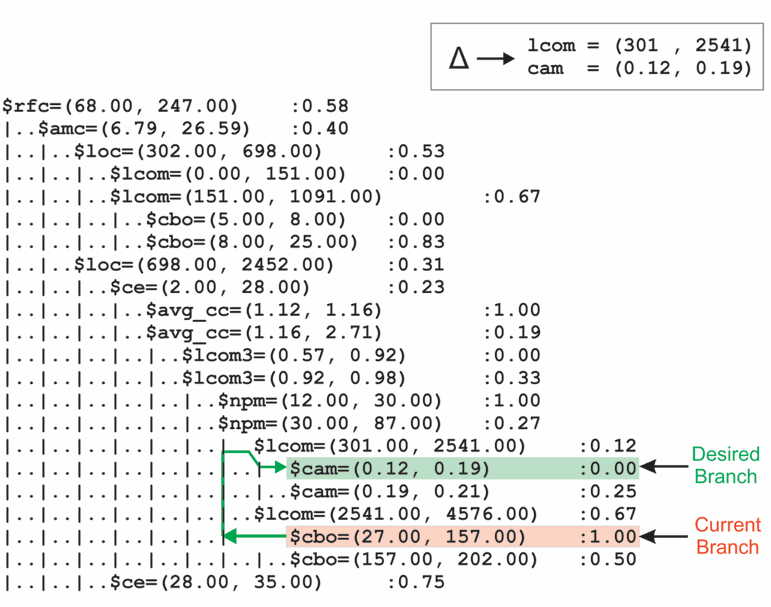
\includegraphics[width=\linewidth]{figs/XTREE_samp.png}
\caption{Sample plans from XTREE. This
tree can be read like a nested if-then-else statement. For
example, lines 3 and 8 show two branches for lines of code
(denoted here as {\em \$loc}) below 698 and above 698.
Any line with a colon ":" character  shows
a leaf of this nesting. For example, if some new code module
is passed down this tree and 
falls to the  line marked in orange,
the colon on that line indicates a 
prediction that this module has a 100\% chance of being defective.
XTREE looks for a nearby branch that has a lower chance of being
defective.
Finding the green branch, XTREE a bad smell threshold
for that module that is the delta between 
the orange branch and the green branch. In this case, that threshold
relates to 
lines of code and comments ({\em lcom}) and the cohesion between 
classes ({\em cam}:   measures similarity of
parameter list to assess the relatedness among the methods of class).
\label{fig:xtree_samp}
\end{figure}




  While not usually labelled as such, ID can
  be viewed as a clustering algorithm that groups together code modules
  with similar defect counts and some shared ranges of code metrics.
  XTREE is a post-processor to ID that reports the delta between 
  nearby groups with different defect counts. \fig{xtree_samp} offers
  a small example of that reflection. In this example:
  \begin{itemize}
      \item Some project has a table of data describing its  classes in the form of \fig{ck}.
      \item After code inspections and running test cases or operational
      tests, each such class is augmented with a defect count.
      \item CART takes that table of data and, using iterative dichotomization,
      it generated the tree of \fig{xtree_samp}.
      \item Once the tree is built, some test case arrives and is passed
      down the tree to a leaf note (see the orange line in \fig{xtree_samp}.
      \item XTREE then looks for a nearby leaf node with a lower defect
      count (see the green line in \fig{xtree_samp}. XTREE bad smell
      thresholds for that method is then the difference between 
      green and orange.
  \end{itemize}
  
  
\subsubsection{XTREE: the details}

 {\em Step1:} Using the training data,  XTREE uses iterative dichotomization to
  divide a table of $N$ code modules  into  groups of
size $\alpha=\sqrt{N}$.

{\em Step2:} For each test code module, 
	  find the {\em current } leaf: take each test , run it down to a leaf in the decision tree.  
After that,	  find the {\em desired} leaf:
		\begin{itemize}[leftmargin=3mm]
		\item Starting at {\em current}, ascend the tree $lvl\in \{0,1,2...\}$ levels;
		\item Identify {\em sibling} leaves; i.e. leaf clusters that can be reached from level $lvl$ that are not same as {\em current }
		\item Using the {\em score} defined above, find the {\em better} siblings; i.e. those with a {\em score} less than $\gamma=0.5$ times the mean score of {\em current}. 
		   If none found, then repeat for $lvl += 1$. Also,
		    return no plan if the new $lvl$ is above the root. 
		\item  Return the {\em closest} better sibling where distance is measured between the mean centroids of that sibling and {\em current}
		\ei
	 Also, find the {\em delta}; i.e. the set difference between  conditions in the decision tree branch to {\em desired} and {\em current}. To find that delta: 
	 \begin{itemize}
	     \item For discrete attributes, delta is the value from {\em desired};
	     \item For  numerics, delta is the numeric difference;
	     \item For numerics  discretized into ranges, delta is a random number selected from the low and high boundaries of the that range.
	     \end{itemize}
	     The bad smell threshold for this module is the delta that would move
	     it from the current to desired lead.
	       
	     



  


\section{Oracles}
\label{sect:eval}
\begin{figure*}[!t]
	\small
	\begin{center}
		\begin{minipage}{.46\linewidth}
			\begin{tabular}{r@{~}|l@{~}|r@{~}|l@{~}|r@{~}|r@{~}|} \cline{2-6}
			 
				
				& \multicolumn{5}{c|}{ Data set  properties}\\ 
			 
				& \multicolumn{2}{c|}{training}   & \multicolumn{3}{c|}{testing}      \\ \cline{2-6}
				data set      & versions           & cases & versions     & cases    & \% defective             \\ \hline
				jedit    & 3.2, 4.0, 4.1, 4.2 & 1257      & 4.3          & 492          & 2 \\
				ivy      & 1.1, 1.4           & 352       & 2.0          & 352          & 11 \\
				camel    & 1.0, 1.2, 1.4      & 1819      & 1.6          & 965          & 19 \\
				ant      & 1.3, 1.4, 1.5, 1.6 & 947       & 1.7          & 745          & 22 \\
				synapse  & 1.0, 1.1           & 379       & 1.2          & 256          & 34 \\
				velocity & 1.4, 1.5           & 410       & 1.6          & 229          & 34 \\
				lucene   & 2.0, 2.2           & 442       & 2.4          & 340          & 59 \\
				poi      & 1.5, 2, 2.5        & 936       & 3.0          & 442          & 64 \\
			 xerces   & 1.0, 1.2, 1.3      & 1055      & 1.4          & 588          & 74  \\ 
			 log4j    & 1.0, 1.1           & 244       & 1.2          & 205          & 92   \\
			 xalan    & 2.4, 2.5, 2.6      & 2411      & 2.7          & 909          & 99  \\\hline 
				
				
			\end{tabular}\end{minipage}\begin{minipage}{.4\linewidth}
			\begin{tabular}{|rrr|rrr|rr|l} \cline{1-8}
			 
				\multicolumn{8}{|c|}{  Results from learning}\\
			 
				\multicolumn{3}{|c|}{untuned} & \multicolumn{3}{c|}{tuned} & \multicolumn{2}{c|}{change}\\
				\cline{1-8}
				
				pd & pf & good? & pd & pf & good? & pd & pf\\\cline{1-8}
				\rowcolor{celadon}55 & 29 &   & 64 & 29 & y & 9 & 0&$\star$\\
				\rowcolor{celadon}	65 & 35 & y & 65 & 28 & y & 0 & -7&$\star$\\
				49 & 31 &   & 56 & 37 &   & 5 & 6\\
				\rowcolor{celadon}	49 & 13 & y & 63 & 16 & y & 14 & 3&$\star$\\
				45 & 19 &   & 47 & 15 &   & 2 & -4\\
				78 & 60 &   & 76 & 60 &   & -2 & 0\\
				56 & 25 &   & 60 & 25 & y & 4 & 0\\
				\rowcolor{celadon}	56 & 31 &   & 60 & 10 & y & 4 & -21&$\star$\\
			\rowcolor{lavenderpink}	30 & 31 &   & 40 & 29 &   & 10 & -2&$\times$\\
				\rowcolor{lavenderpink}32 & 6 &   & 30 & 6 &   & -2 & 0&$\times$\\
				\rowcolor{lavenderpink}38 & 9 &   & 47 & 9 &   & 9 & 0&$\times$\\
				\hline 
			\end{tabular}
			
		\end{minipage}
	\end{center}    
	
	\caption{Training and test {\em data set properties} for  Jureczko data ,
		sorted by \% defective examples.
		On the right-hand-side, we show the {\em results from learning}.
		Data is usable if it has a recall of 60\% or more and false alarm of 30\% or less (and note that, after tuning, there are more usable data sets than before). Results  	\colorbox{celadon}{ marked with ``$\star$''} show large improvements in performance, after tuning
		(lower {\em pf} or higher {\em pd}).
		Data in  the  \colorbox{lavenderpink}{three bottom rows}, marked with ``$\times$'', are  performing
		poorly-- that data so few non-defective examples  that it  is hard for
		our learners to distinguish between classes.
	}\label{fig:j}
\end{figure*}


As highlighted previously, there are several detection techniques for anti-patterns, yet these fail to address the issue of checking the proposed changes for their efficacy. Much of the refactoring needs to evaluated for their usefulness. To this end, there needs to be an oracle, a procedure that can be employed to distinguish between good and bad options. The dearth oracles is not unique to this domain, for instance a recent survey by Barr et al \cite{barr15}

Our strategy (discussed in greater detail below) divides this data into a training and a testing set. The purpose of training set is twofold: (1) We apply a data miner to construct an oracle that acts as a quality predictor; (2) We build the planners to reason across the data. 

Next, we employ the planners to generate plans to improve the quality of defective classes in the test set. In addition to the plans obtained from our planners we may have some common refactoring options that the developers tend to use. The oracle built previously can be used to assess the the changed examples and this can be used to compare refactoring operations.

It's worth noting that this approach depends on having effective oracles for assessing the results. It proved to be more complicated to commission the Jureczko data sets for this study. For that data, we found that the quality predictors built from this data are far from perfect; However, for some data sets, the  predictors could be salvaged using the techniques discussed in this section.

\fig{j} shows our preliminary studies with the Jureczko data. Given access to $V$ released versions, we test on version $V$ and train on the available data from $V-1$ earlier releases (as shown in \fig{j}, this means that we are training on hundreds to thousands of classes and testing on smaller test suites). Note the   \colorbox{lavenderpink}{three bottom} \colorbox{lavenderpink}{rows}   marked with $\times$: these contain predominately defective classes (two-thirds, or more).  In such data sets, it is hard to distinguish good from bad (since there are so many bad examples). 

In order to identify the presence (or absence) of defects, we can consider using Boolean classes in the  Jureczko data ( \texttt{True} if defects $\gt$ 0; \texttt{False} if defects = 0). For such data, quality of the predictor can be measured using (1) the  probability of detection (a.k.a. ``pd'' or recall):  the percent of faulty classes in the test data detected by the {\em predictor}; and (2) the  probability of false alarm (a.k.a. ``pf''): the percent of non-fault classes that are {\em predicted} to be defective.

As a preliminary study, we split the Jureczko  data into train and test groups. Random Forest (again, from the SciKit learn kit~\cite{Pedregosa2012}) was built from the training data, then applied to the test data. The ``untuned'' columns of \fig{j} shows those results. We called a data set ``usable'' if Random Forest was able to classify majority of the instances correctly. For this purpose, we set a threshold of $\mathit{pd}\ge 60 \wedge \mathit{pf} \le 30$\% to select suitable data sets. With this threshold, however, none of our data sets were be suitable for this study.

Fortunately, the ``tuned'' columns of \fig{j} show that we can salvage some of the data sets. Pelayo and Dick~\cite{pelayo07} report that defect prediction is improved by SMOTE~\cite{Chawla2002}; i.e. an over-sampling of minority-class examples and an under-sampling of majority-class examples. Also, Fu et al.~\cite{fu:ase15} report that parameter tuning with differential evolution~\cite{storn97} can quickly explore the tuning options of Random Forest to find better settings for the (e.g.) size of the forest, the termination criteria
for tree generation, etc. The rows \colorbox{celadon}{marked with a $\star$} in \fig{j} show data sets whose performance was improved remarkably by these techniques. For example, in {\em poi}, the recall increased by 4\% while the false alarm rate dropped by 21\%. However,  as might have been expected, we could not salvage the data sets in the  three bottom rows.

In summary, while we cannot trust predictors from some of our Jureczko data sets,
we can plan ways to reduce defects in {\em jedit, ivy, ant, lucene} and {\em poi}.
Accordingly, when this study explores the Jureczko data, we will use these five data sets.

(Aside: One important detail to be stressed here is that, when we applied    SMOTE-ing and
parameter tunings, those techniques were applied to the training data and {\em not}
the test data; i.e. we took care that no clues from the test set were ever used in this tuning process.)





 


\subsection{Need for Planning}
During lifecycle, a software system undergoes continuous changes in order to keep up with the business level demands \cite{lehman79}. Unfortunately, due to market/customers constraints, the source code quality is often neglected with the risk of introducing \textit{code bad smell} (or code-smells) \cite{fowler09}. Code smells are symptomatic of design issues in codes like code understandability and code changeability. If left unaddressed, these can lead to a variety of maintenance problems and faults in software systems \cite{fowler09}\cite{marinescu06}. Fowler \cite{fowler09} and Brown et al. \cite{brown98} defined a catalogue of more than 30 anti-patterns. It is a common notion that the critiques motivated by anti-patterns and code smells would be more comprehensible to developers because many code smells are associated with conventional refactoring operations. 

The choice of refactoring operations to address the code smells arise from strongly held beliefs of developers on these topics, and their beliefs in turn are motivated by personal experiences. 

The distinction between developers' beliefs and empirical findings is particularly profound in the case of code smells. For instance, \cite{abbes11} showed that the presence of an anti-pattern in the source code does not decrease the developers' performance, while a combination of anti-patterns results in a significant decrease of their performance \cite{abbes11}\cite{yama13}. While the results of this study indicates that single anti-patterns are not harmful, they also reveals that anti-patterns are quite diffuse in software systems and very often code components are affected by more than one anti-pattern. In addition, we have empirical evidence that the number of anti-patterns in software systems increases over time and only in few cases they are removed through refactoring operations \cite{arcoverde11}\cite{chatzigeorgiou10}. Additionally, Yamashita and Moonen\cite{} observed that several developers did not take conscious actions to alleviate bad smells that were present in the code. 

Closer inspection revealed that this is not due to the lack of relevance of code smells, but a number of other factors, like: (1) lack of awareness; (2) More importantly, lack of developer friendly tools \cite{}. The study goes on to show that these developers are in need of better support tools that assist them during the software evolution cycle.  Specifically, developers needed tools to (1) be developer friendly; (2) be operable in real-time; and (3) be capable of identifying problematic areas using error prediction.

Therefore to assist developers in their refactoring efforts by providing them with reliable analytics it is useful to have automatic methods that can augment human expertise (or replace them if such experts are absent) in addition to offering a second opinion. Accordingly, the rest of this paper defines and evaluates automatic methods to address the above issues.
  

\subsection{What is a ``Plan''?}
To address the issues discussed in the previous section, we conjecture that the planners must generate valid and meaningful refactoring operations, we refer to these as \textit{plans}. These plans are synthesized by the planner and are thus unique in that they are agnostic to any prior notions of the developers in addition to them being local to the software project being refactored.  

To do this, our planners use tables of data with independent features and a dependent class feature. Classes have weights  that  indicate  what rows are ``bad'' or ``better''. Plans  change   a row such that it is more likely to be ``better''. Specifically, for every test example $Z$,   planners proposes a  plan $\Delta$ to adjust   feature $Z_j$:

{\small\[
\forall \delta_j \in \Delta :  Z_j =  
\begin{cases}
     Z_j + \delta_j& \text{if $Z_j$ is numeric}\\
    \delta_j              & \text{otherwise}
\end{cases}
\]}

For example, to simplify a  large bug-prone  method, our planners might suggest to a developer to reduce its size (i.e.  refactor that code by, say, splitting it across two simpler functions).

Additionally, if a developer were to suggest a specific refactoring option, our planners can query the option and report on its possible usability. Note that we make no assumption that a plan mentions every feature (so plan1 can be  more succinct than plan2 when plan1  mentions fewer features than plan2).


\section{Test Data}\label{sect:tesd}

To assess our planning methods, our data (see git.io/vGYxc) comes from Jureczko et al.'s object-oriented JAVA systems~\cite{jureczko10}.

The Jureczko data records the number of known defects for each class using a post-release bug tracking system. The classes are described in terms of nearly two dozen metrics, included in the Chidamber and Kemerer metric suite, such as number of children (noc), lines of code (loc), etc. For details on the Jureczko data, see  \fig{ck}. All the planning methods of this paper reflect on the numeric value of the raw defect counts to estimate the quality of the class. The predictor considers defects to be a Boolean class data set, where defects are \texttt{TRUE} if the numeric defect count is greater than zero and \texttt{FALSE} otherwise. The choice of this data set was is based on the taxonomy of the smells, in which we focus on the measurable properties needed to detect a given smell. This set of metrics is not restricted and can be easily extended with other metrics.




	\begin{figure} 
	\begin{shaded}
  ~\hrule~
  
 {\bf Figure 7.A: Measuring Variability} 
	
	For  continuous and discrete values,
the {\em variability} can be measured using standard deviation $\sigma$ or entropy $e$.
Note that \mbox{$\sigma = \sqrt{\sum^n_{i=1} \left( \frac{(x_i - \bar{x})^2}{n-1}\right)}$}
where $\bar{x}$ is the mean of  numeric features $x_1,x_2,..x_n$.
Also \mbox{$e = - \sum^n_{i=1} p_i \mathit{log}_2(p_i)$} 
for  $n$ discrete values  at frequency
$f_1,f_2,.. f_n$ for \mbox{$N = \sum^n_{i=1} f_i$} and $p_i = f_i/N$.

  ~\hrule~
	
	{\bf Figure 7.B: Measuring distance}
	
	We use
		 Aha et al.'s standard Euclidean distance measure~\cite{aha91}.  For $F$ independent features, the measure returns   $d(X,Y)=\sqrt{\sum_i^F  w_i\Delta(X_i,Y_i)^2}$. Here, $w_i$ is a weight term for each feature
		 (usually set to 1).
			Within $\Delta$, if   $X_i,Y_i$ are both missing  values, then  return 1.
			Otherwise, replace any  missing items with values that maximizes the following.
			For numerics, $\Delta$ normalizes $X_i,Y_i$ (to the range 0,1 for min,max) then
			returns 
			$X_i - Y_i$. For discrete variables, $\Delta$ returns 0,1 if $X_i,Y_i$ are the
			same,different (respectively).  

 ~\hrule~
 
	{\bf Figure 7.C: Top-down Clustering with WHERE}
	
				WHERE  divides data into  groups of size $\alpha=\sqrt{N}$. 
		Using this measure, WHERE runs as follows:
		\begin{enumerate}[leftmargin=3mm]
			\item Find   two   distance cases,  $X,Y$
			by picking any case $W$ at random, then setting $X$ to its most
			distant case, then setting $Y$ to the case most distant from
			$X$
			(which requires only $O(2N)$ comparisons).
			\item Project each case $Z$
			to position $x$ on a    lines running from $X$ to $Y$: if $a,b$  are distances  $Z$ to $X,Y$  then  $x = (a^2+c^2 - b^2)/(2ac)$.
			\item Split the data at the median $x$ value of all cases.
			\item For   splits larger than  $\alpha=\sqrt{N}$, recurse from step1.
		\end{enumerate}
 In terms of related work,
	  the above is similar in approach to Boley's PDDP algorithm~\cite{boley98}, but PDDP requires an $O(N^2)$ calculation
	  at each recursive level to find the PCA principle component. Our method, on the other hand,
	  performs the same task with only $O(2N)$ distance calculations 	using the 
	  FASTMAP heuristic~\cite{Faloutsos1995} shown in step1. Platt~\cite{platt05} notes that FASTMAP is a  Nystr\"om approximation to the first component of PCA.  
	  
	   ~\hrule~
	   
	{\bf Figure 7.D: Top-down division with Decision Trees}
	
	Find a split in the values of  independent features that most reduces the variability
  of the dependent feature (measured using \fig{where}.A). Construct a standard decision tree using these splits.
	
	 ~\hrule~
	 
	 	{\bf Figure 7.E: Finding the most informative rows}
	

Discretize all numeric features using the Fayyad-Iranni discretizer~\cite{FayIra93Multi}
(divide numeric columns into bins $B_i$, each of which  select for the fewest cluster ids).
Let feature $F$ have bins $B_i$, each of which contains $n_i$ rows
and 
let each bin $B_i$ have entropy $e_i$ computed from the frequency of clusters seen in that bin (computed from \fig{where}.A).
Cull the the features as per~\cite{papa13}; i.e. just use the $\beta=33\%$ most informative features
where  the   value of  feature $F$ is $\sum_i e_i\frac{n_i}{N}$ ($N$ is the number of rows).

~\hrule~ 

	  \end{shaded}
		\caption{Some algorithms used in this paper.}\label{fig:where}
		\end{figure}
  
\section{Planning Methods}\label{sect:planners}
 
In this we describe the planners used in our study. First, we reintroduce a planner called CD which was an outcome of our previous work~\cite{me12c} which generates plans using a top-down bi-clustering method described in \fig{where}.C to recursively partition the data along the dimension that captures the greatest variability in the data. Then, we present XTREE, a novel planner introduced in this work, which uses a decision tree learner \fig{where}.D for planning.

% This section describes the new XTREE planner and a planner called CD which was an outcome of our previous work~\cite{me12c}. XTREE, a novel planner introduced in this work,  uses the decision tree learner of \fig{where}.D.

Both methods aim to address the issues highlighted in \tion{prelim}. To achieve this: (1)~they find plans, which can be use to generate reliable refactoring options, particular to each test case by reflecting on local data; and (2)~they offer a mechanism for critiquing bad refactoring options.

% (i) generating reliable refactoring options, and (ii) critiquing bad refactoring options. 

\subsection{  Methods}

Our  description of the methods adopts the following convention. All variables set via  our engineering judgement  with Greek letters; e.g. $\alpha,\beta,\gamma,\omega$. In this paper, we show our current settings to these variables produces useful results. Elsewhere \cite{krall14,fu:ase15}, we are exploring tuning methods to find better settings but  we have nothing definitive yet to report on auto-tuning planners.

\subsubsection{Centroid Deltas (CD)}

% Method1 computes a plan from the difference between where you are  (which we will call $C_i$) and where you want to be (which we will call $C_j$).

Large data sets can be adequately represented by a few dozen (or so) clusters, and meaningful inferences can be drawn from the centroids of these clusters. This method generates plans for improving faulty classes by looking at the difference between the cluster centroid that most closely resembles the defective class from the training data (denoted by $C_i$) and the cluster centroid that represents a better, non-defective, class (denoted by $C_j$).
 
To do this, CD clusters training data based on the independent variables using the WHERE algorithm of \fig{where}.C and replaces all clusters with their centroids computed from the median value of each continuous/discrete feature. Then, for every cluster $C_i$ it finds the closest centroid $C_j$ that has a better performance score. For Jureczko data, ``better'' means fewer defective examples. CD then caches the delta between the independent features of $C_i$ and $C_j$. For continuous features, this delta is $C_j - C_i$. Finally, for every test case, CD uses the distance measure $d$ shown in \fig{where}.B to find the nearest centroid $C_i$.  It then proposes a plan for improving that test case: the conjunction of all the deltas between $C_i$ and $C_j$.

\begin{figure}[t] 
	\begin{shaded}
  ~\hrule~
	
Using the training data,  divide the data using the decision tree algorithm of \fig{where}.D into groups of
size $\alpha=\sqrt{N}$.
For test item, 
	  find the {\em current } leaf: take each test instance, run it down to a leaf in the decision tree.  
After that,	  find the {\em desired} leaf:
		\begin{itemize}[leftmargin=3mm]
		\item Starting at {\em current}, ascend the tree $lvl\in \{0,1,2...\}$ levels;
		\item Identify {\em sibling} leaves; i.e. leaf clusters that can be reached from level $lvl$ that are not same as {\em current }
		\item Using the {\em score} defined above, find the {\em better} siblings; i.e. those with a {\em score} less than $\gamma=0.5$ times the mean score of {\em current}. 
		   If none found, then repeat for $lvl += 1$. Also,
		    return no plan if the new $lvl$ is above the root. 
		\item  Return the {\em closest} better sibling where distance is measured between the mean centroids of that sibling and {\em current}
		\ei
	 Also, find the {\em delta}; i.e. the set difference between  conditions in the decision tree branch to {\em desired} and {\em current}. To find that delta: (1)~for discrete attributes, delta is the value from {\em desired}; (2)~for  numerics, delta is the numeric difference; (3)~for numerics  discretized into ranges, delta is a random number selected from the low and high boundaries of the that range.
	 
		Finally, return the delta as the plan for improving the test instance.
		~\hrule~
		\end{shaded}
		\caption{XTREE}		\label{fig:xtrees_bare}
	\end{figure}



\subsubsection{XTREE}

A potential problem with CD is the {\em unsupervised} nature of the clustering algorithm (WHERE) that executes without knowledge of the target class. It would be beneficial for us to use {\em Supervised} methods that also reflect on the target class.

XTREE was developed to address this problem. It uses a supervised decision tree algorithm of \fig{where}.D to categorize the data Next, XTREE devises plans from the branches of the decision trees using the code of \fig{xtrees_bare}. That code asks three questions, the last of which returns the plan:

\be
\item What {\em current} branch does a test case fall in?
\item What {\em desired} branch would the test case want to move to?
\item What are the {\em deltas} between current and desired? 
\ee

In finding the answers to the above questions, XTREE can (a) Generate an wealth of plans (that can be potential refactoring operations); (b) Critique plans based on their location in the decision tree constructed. In addition to the above, XTREE also offers developers a visual medium to validate their proposals for refactoring, see ~\fig{xtree_samp}.

\begin{figure}[btp!]
\centering
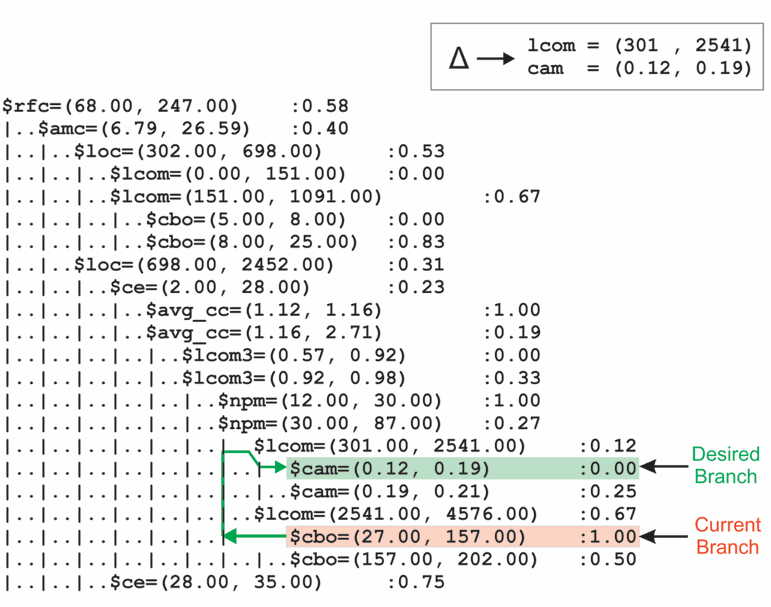
\includegraphics[width=\linewidth]{figs/XTREE_samp.png}
\caption{Sample plans from XTREE}\label{fig:xtree_samp}
\end{figure}


\section{Experiments}

This section describes an experimental design (and results) for evaluating the above four methods. 
\subsection{Experimental Design}

\subsubsection{A Strategy for Evaluating Planners}
 
Our experimental design is shown in \fig{design}. We divide the
project data  into two disjoint sets {\em train} and {\em test}
(so \mbox{{\em train} $\cap ${\em test} $=\;\emptyset$}).
Next, from the train set, we build both a {\em planner} and
 a {\em  predictor}. 

Our general framework does not   commit to any particular choice of { planner} or { predictor} but, for the purposes of this paper:
\bi
\item Our {\em planners} will be XTREE and CD;
\item Our  {\em predictor} will be the Random Forest Classifier~\cite{Breiman2001} (for discrete classes) and Random Forest Regressor (for continuous classes) taken from  SciKit Learn~\cite{Pedregosa2012}.   We use these
data miners since extensive studies have shown these to be amongst the better alternatives for mining software data~\cite{lessmann}.
\ei
As for the {\em test} data, this is passed to the { predictor}
to measure performance statistics related to effectiveness. 

If our { predictors} fail to perform effectively on the test data,
then we cannot trust them to comment on our plans. Accordingly,
if that performance is unsatisfactory, we abort. Recall from \tion{tesd} that this step indicated
we should not use some of the  Jureczko data.

Else, we (1)~apply the { planner} to alter the {\em test} data;
then (2)~apply the { predictor} to the altered data $test'$;
then (3)~return data on the {\em before, after} predictions expressed as percent improvement, denoted by  $R=(1-\frac{\mathit{after}}{\mathit{before}})\times100\%$, with the following following properties:
\bi
\item If $R  = 0\%$, this means  ``no change from baseline''; 
\item If $R \gt 0\%$, this indicates ``

improvement over the baseline'';
\item If $R \lt 0\%$, this indicates ``optimization failure''.
\ei

\begin{figure}[!t]
{\small 
\[
\begin{array}{r} 
\mathrm{project}\\
\mathrm{data}
\end{array} 
\left\{\begin{array}{l}\mathit{train}
        \left\{\begin{array}{l}
                \mathrm{learn\;a\;}\mathrm{predictor\;}\mathrm{(e.g.\;via \;Random\;Forest)}\\
                \mathrm{learn\;a\;}\mathrm{planner\;}\mathrm{(e.g.\;via \; XTREE)}
              \end{array}\right.
       \\
      ~\\
\mathit{test}  
    \left\{\begin{array}{l@{~}l}
           \mathit{before}& =\mathrm{Performance\; scores \hspace{2pt} in \hspace{2pt}}\mathit{test}\\
           \mathrm{\bf if\;}\mathit{before} & >  \mathit{0}\\
           \mathrm{\bf then} &
           \left\{
            \begin{array}{l}
                \mathit{test'} = \mathrm{planner}(\mathit{test})\\
                \mathit{after} =\mathrm{predictor}(\mathit{test'})\\ 
                \mathrm{{\bf return}\;} R=(1-\frac{\mathit{after}}{\mathit{before}})\times 100 \%
            \end{array}
          \right.
   \end{array}\right.
\end{array} \right. 
\]}
 \caption{Experimental design .}\label{fig:design}
 \end{figure}



\subsubsection{Statistical Methods}
Our methods use some stochastic algorithms; e.g. WHERE's selection of ``what example to explore first'' (see \fig{where}.C) and XTREE' occasional use of a random guess when deciding what part of a discretized range to include in the plan (see \fig{xtrees_bare}). Hence, we report the $R$ values seen in 40 repeated runs, with different random number seeds (we use 40 since that is  more than the 30 samples  needed to satisfy the central limit theorem).

To rank our methods using the results from these 40 repeats, we use the Scott-Knott test recommended by Mittas and Angelis~\cite{mittas13}. 

In accordance to that test, using the median values of each method, we
sort a list of  $l=40$ values of $R$ values found in  $ls=4$ different methods. 
Then, we split $l$ into sub-lists $m,n$ in order to maximize the expected value of differences  in the observed performances before and after divisions. E.g. for lists $l,m,n$ of size $ls,ms,ns$ where $l=m\cup n$: \[E(\Delta)=\frac{ms}{ls}abs(m.\mu - l.\mu)^2 + \frac{ns}{ls}abs(n.\mu - l.\mu)^2\]

We then apply a apply a statistical hypothesis test $H$ to check
if $m,n$ are significantly different  (in our case, the conjunction of A12 and bootstrapping). If so, Scott-Knott recurses on the splits. In other words, we divide the data if \textit{both} bootstrap sampling and effect size test agree that a division is statistically significant (with a confidence of 99\%) and not a small effect ($A12 \ge 0.6$).

For a justification of the use of non-parametric bootstrapping, see Efron \& Tibshirani~\cite[p220-223]{efron93}. For a justification of the use of effect size tests see Shepperd\&MacDonell~\cite{shepperd12a}; Kampenes~\cite{kampenes07}; and Kocaguenli et al.~\cite{Kocaguneli2013:ep}. These researchers warn that even if a hypothesis test declares two populations to be ``significantly'' different, then that result is misleading if the ``effect size'' is very small. Hence, to assess the performance differences we first must rule out small effects using A12, a test   recently endorsed by Arcuri and Briand at ICSE'11~\cite{arcuri11}.



\subsubsection{Report Format}

   
Our results are presented in the form of line diagrams like those shown on the right-hand-side of the following example table.
The black dot shows the median $R$ value and the horizontal likes stretch 
from the 25th percentile to the 75th percentile (a region called the inter-quartile
range, or IQR).

\begin{center}

{\small Example \begin{tabular}{{l@{~~~}l@{~~~}r@{~~~~}r@{~~~}c@{}r}} 
\arrayrulecolor{lightgray}
\rowcolor{lightgray}\textbf{Rank} & \textbf{Treatment} & \textbf{Median} & \textbf{IQR} & \\
1 &      XTREE &    62  &  6 & \quart{47.2}{4.8}{49.6}{115}  \\
\hline 2 &      CD &    44  &  18 & \quart{28}{14.4}{35.2}{115} \\
\hline \end{tabular}}
\end{center}

In this example table, the rows are  sorted on the median values of each method. Note that all the methods have $R\gt0\%$; i.e. all these methods reduced the expected value of the performance score in that experiment while XTREE achieved the greatest reduction (of 62\% from the original value).

The above example table has a  left-hand-side  {\bf Rank} column, computed using the
Scott-Knott test described above. In this example table, XTREE is ranked the best, while CD and CD+FS together are ranked the worst.

\subsubsection{Other Details}
 
\fig{jur} shows the effectiveness of our methods seen in 40 repeats with each data set.
In these experiments,   the dependent variables of Jureczko data set is discrete. Hence, while choosing the predictor, we used Random Forest as a classifier for Jureczko data.

The Jureczko data, being temporal in nature, allows us to implement a validation procedure that ensures only past data is ever used to predict future values. Hence, in that data, we used the train/test sets shown in \fig{j}. (Aside: note  that all the SMOTE-ing and Random Forest tunings (discussed in \tion{tesd}) occurred in the {\em train} phase of \fig{design}).

\begin{figure}[!t]
%{\scriptsize \textbf{Ant}\\[0.1cm]}

{\scriptsize \textbf{Ant}~~~~~~~~ \begin{tabular}{{l@{~~~~}l@{~~~~}r@{~~~~}r@{~~}c@{}r}}
\arrayrulecolor{lightgray}
\rowcolor{lightgray}\textbf{Rank} & \textbf{Treatment} & \textbf{Median} & \textbf{IQR} & \\
  1 &         XTREE &    56   &  21  & \quart{54}{25}{65}{1} \\
\hline  2 &        Alves &    32   &  17  & \quart{28}{20}{37}{1} \\
\hline  3 &     Shatnawi &    15   &  4 2 & \quart{15}{6}{18}{1} \\
  3 &           CD &    12   &  0  & \quart{15}{0}{15}{6} \\
\hline \end{tabular}}\\

%{\scriptsize \textbf{Lucene}\\[0.1cm]}
%{\scriptsize \textbf{Poi}\\[0.1cm]}
{\scriptsize \textbf{Poi}~~~~~~~~ \begin{tabular}{{l@{~~~~}l@{~~~~}r@{~~~~}r@{~~}c@{}r}}
\arrayrulecolor{lightgray}
\rowcolor{lightgray}\textbf{Rank} & \textbf{Treatment} & \textbf{Median} & \textbf{IQR} & \\
        1 &         XTREE &    20   &  16  & \quart{39}{40}{51}{2} \\
\hline  2 &        Alves &    14   &  16  & \quart{21}{41}{37}{2} \\
\hline  3 &           CD &    11   &  0  & \quart{23}{0}{23}{7} \\
        3 &     Shatnawi &    8   &  1  & \quart{19}{5}{21}{2} \\
\hline \end{tabular}}\\

{\scriptsize \textbf{Lucene}~ \begin{tabular}{{l@{~~~~}l@{~~~~}r@{~~~~}r@{~~}c@{}r}}
\arrayrulecolor{lightgray}
\rowcolor{lightgray}\textbf{Rank} & \textbf{Treatment} & \textbf{Median} & \textbf{IQR} & \\
        1 &         XTREE &    16   &  6  & \quart{50}{29}{71}{4} \\
        1 &     Shatnawi  &    15   &  2  & \quart{63}{10}{67}{4} \\
\hline  2 &           CD  &    13   &  0  & \quart{55}{0}{55}{6} \\
\hline  3 &        Alves  &    9   &  4  & \quart{33}{19}{42}{4} \\
\hline \end{tabular}}\\


%{\scriptsize \textbf{Ivy}\\[0.1cm]}
{\scriptsize \textbf{Ivy}~~~~~~~~ \begin{tabular}{{l@{~~~~}l@{~~~~}r@{~~~~}r@{~~}c@{}r}}
\arrayrulecolor{lightgray}
\rowcolor{lightgray}\textbf{Rank} & \textbf{Treatment} & \textbf{Median} & \textbf{IQR} & \\
        1 &        Alves &    67   &  20  & \quart{58}{21}{71}{1} \\
\hline  2 &         XTREE &    52   &  22  & \quart{42}{24}{55}{1} \\
\hline  3 &           CD &    35   &  0  & \quart{27}{0}{27}{2} \\
\hline  4 &     Shatnawi &    20   &  7  & \quart{18}{8}{21}{1} \\
\hline \end{tabular}}\\

%{\scriptsize \textbf{Jedit}\\[0.1cm]}

{\scriptsize  \textbf{Jedit}~~~~~~~ \begin{tabular}{{l@{~~~}l@{~~~~}r@{~~~~}r@{~~}c@{}r}}
\arrayrulecolor{lightgray}
\rowcolor{lightgray}\textbf{Rank} & \textbf{Treatment} & \textbf{Median} & \textbf{IQR} & \\
  1 &        Alves &    36   &  7  & \quart{60}{10}{66}{1} \\
  1 &        XTREE &    36   &  0  & \quart{66}{0}{66}{2} \\
  1 &     Shatnawi &    36   &  9  & \quart{53}{13}{66}{1} \\
  1 &          CD &    36   &  0  & \quart{66}{0}{66}{2} \\
\hline \end{tabular}}\\
\caption{Results on  Jureczko   data sets.  Results from 40 repeats.
Values come from \eq{diff}.
Values near 0
imply no improvement,
{\em Larger} median values are {\em better}. }
\label{fig:jur}
\end{figure}

% ## ant

% {\scriptsize \begin{tabular}{l@{~~~}l@{~~~}r@{~~~}r@{~~~}c}
% \arrayrulecolor{lightgray}
% \textbf{XTREE} & \textbf{Treatment} & \textbf{Median} & \textbf{IQR} & \\\hline
%   1 &     Shatnawi &    15.66  &  4.82 & \quart{15}{6}{18}{1} \\
% \hline  2 &        Alves &    32.53  &  17.47 & \quart{28}{20}{37}{1} \\
% \hline  3 &         XTREE &    56.02  &  21.68 & \quart{54}{25}{65}{1} \\
% \hline \end{tabular}}


% ## ivy

% {\scriptsize \begin{tabular}{l@{~~~}l@{~~~}r@{~~~}r@{~~~}c}
% \arrayrulecolor{lightgray}
% \textbf{XTREE} & \textbf{Treatment} & \textbf{Median} & \textbf{IQR} & \\\hline
%   1 &     Shatnawi &    20.0  &  7.5 & \quart{18}{8}{21}{1} \\
% \hline  2 &         XTREE &    52.5  &  22.5 & \quart{42}{24}{55}{1} \\
% \hline  3 &        Alves &    67.5  &  20.0 & \quart{58}{21}{71}{1} \\
% \hline \end{tabular}}


% ## jedit

% {\scriptsize \begin{tabular}{l@{~~~}l@{~~~}r@{~~~}r@{~~~}c}
% \arrayrulecolor{lightgray}
% \textbf{XTREE} & \textbf{Treatment} & \textbf{Median} & \textbf{IQR} & \\\hline
%   1 &     Shatnawi &    36.36  &  9.09 & \quart{53}{13}{53}{1} \\
%   1 &         XTREE &    36.36  &  0.0 & \quart{53}{0}{53}{1} \\
%   1 &        Alves &    45.45  &  27.28 & \quart{39}{40}{66}{1} \\
% \hline \end{tabular}}


% ## lucene

% {\scriptsize \begin{tabular}{l@{~~~}l@{~~~}r@{~~~}r@{~~~}c}
% \arrayrulecolor{lightgray}
% \textbf{XTREE} & \textbf{Treatment} & \textbf{Median} & \textbf{IQR} & \\\hline
%   1 &        Alves &    9.85  &  4.44 & \quart{33}{19}{42}{4} \\
% \hline  2 &     Shatnawi &    15.76  &  2.45 & \quart{63}{10}{67}{4} \\
%   2 &         XTREE &    16.75  &  6.9 & \quart{50}{29}{71}{4} \\
% \hline \end{tabular}}


% ## poi

% {\scriptsize \begin{tabular}{l@{~~~}l@{~~~}r@{~~~}r@{~~~}c}
% \arrayrulecolor{lightgray}
% \textbf{XTREE} & \textbf{Treatment} & \textbf{Median} & \textbf{IQR} & \\\hline
%   1 &     Shatnawi &    8.53  &  1.78 & \quart{19}{5}{21}{2} \\
% \hline  2 &        Alves &    14.95  &  16.38 & \quart{21}{41}{37}{2} \\
% \hline  3 &         XTREE &    20.64  &  16.02 & \quart{39}{40}{51}{2} \\
% \hline \end{tabular}}



\subsection{Experimental Results}

\begin{figure}[tb!]
\centering
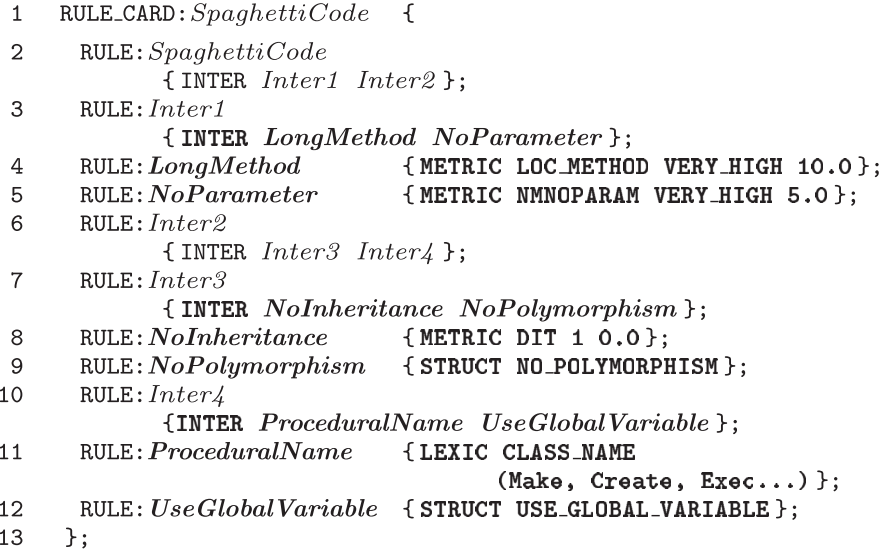
\includegraphics[width=\linewidth]{figs/thresh.png}
\caption{Thresholds used by DECOR to detect Spaghetti Code~\cite{moha10}.}\label{fig:thresh}
\end{figure}

 
Recall from our introduction that we are assessing planners on three criteria:
{\em effectiveness}, which is how much they reduce the expected value of the changed examples;
{\em succinctness}, which is how many things we need to change to achieve a plan;
and {\em insightfulness}, which is how different are the plans from standard truisms.

\begin{figure}[tbp!]
\centering
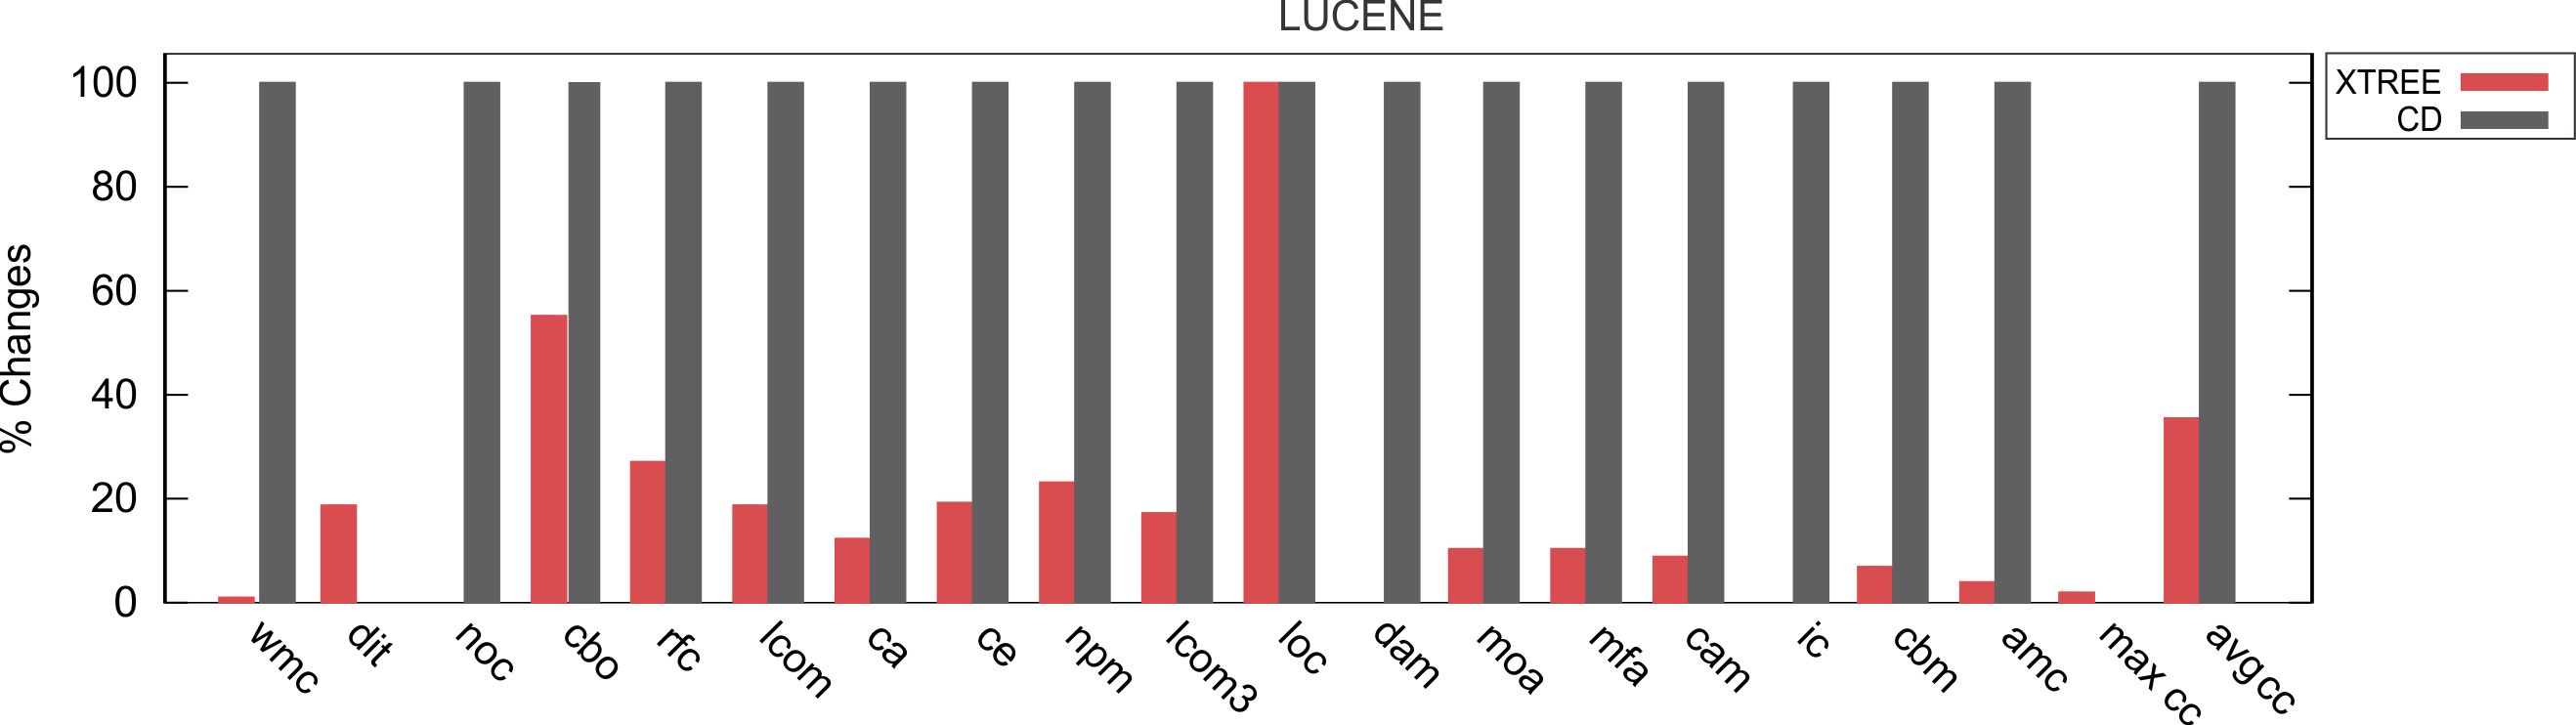
\includegraphics[width=\linewidth]{figs/PercentChanges.png}
\caption{Percent frequency for how often certain feature was changed by a plan.}\label{fig:changed}
\end{figure}


\begin{figure*}[!y]
\centering
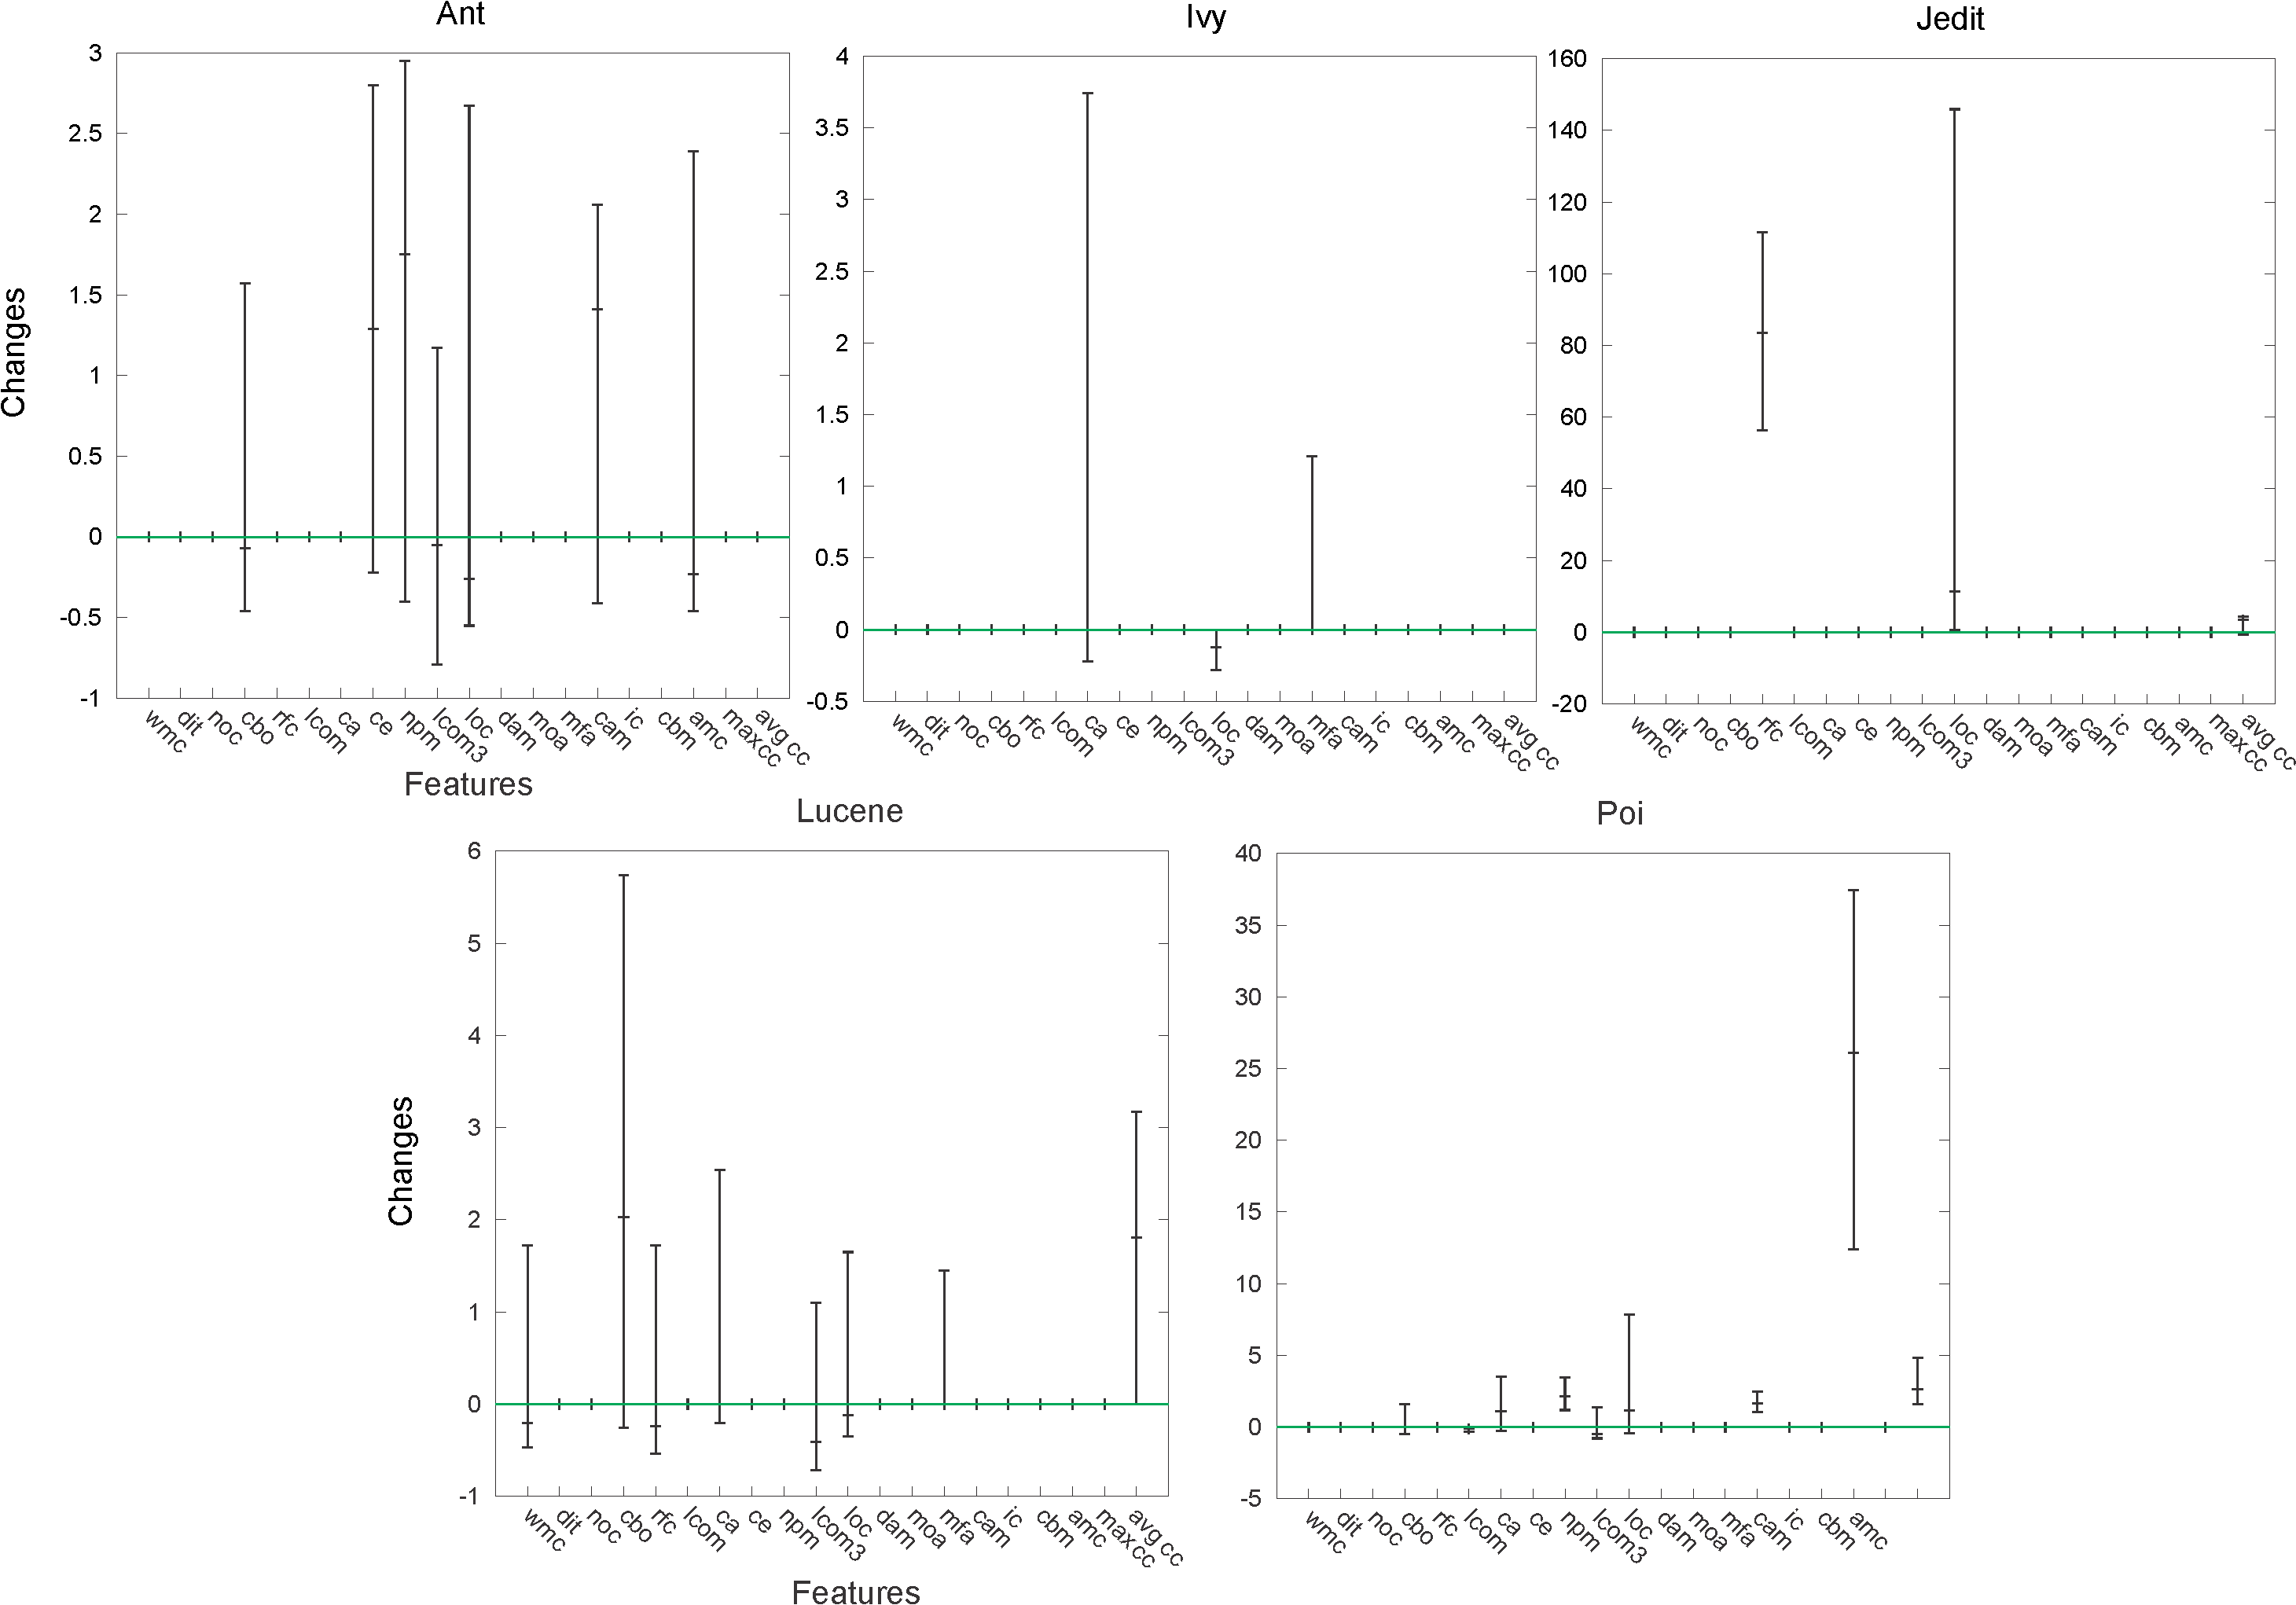
\includegraphics[width=0.90\linewidth]{figs/changes0.png}
\caption{Suggested Changes}
\label{figs:changes}
\end{figure*}

\subsubsection{RQ1: Can a planner suggest plans to improve the quality ofa defective class?}

Measured in terms of effectiveness, some data sets were harder to optimize than others. However, in most data sets, large reductions were observed. We noticed an improvement of 85.54\%, as compared to the original baseline in Ant and 36.36\% in Lucene, \fig{jur}.

Overall, XTREE was most the effective. It was the top-ranked method in 3 cases and performed just as well in the other two. Where it ranked better, it had significant improvements in the median performance values. In the Jureczko data sets, there was an improvement of at least 25\% compared to our previous method.

\fig{changed} reports the percent of times in the 40 repeats that a method proposed changing a feature. The left-hand-side plot of that figure reports results from one of the Jureczko data sets ({\em lucene}) and the right-hand-side shows a Siegmund data set ({\em BDBJ}). 

In these plots, {\em more} succinct a planning method, {\em fewer} the frequency (in percent) where it recommends changing a particular feature (i.e. the vertical bars in that plot are {\em lower}). For example, XTREE's plans were usually succinct --- in all  data sets, XTREE   changes around a fifth of the features (see \fig{types}). On other hand,  Method1 (CD) was the least succinct  since it  wanted to change all features (observe the change frequencies as high as 100\% for all features). Method1's policy of ``change everything''  might be acceptable if this approach lead to the most effective changes. However, in \fig{jur} there is no evidence for this.  
 

\begin{figure}[!b]
\centering
{\small
\begin{tabular}{l|lrrrr}
  \hline
  \rowcolor{lightgray}
 &       & XTREE & BIC   & CD   &CD+FS \\\hline
&Ant    & 20\% & 87\% & 80\% & 10\%  \\
Jureczko&Ivy    & 21\% & 81\% & 70\% & 20\%  \\
data&Jedit  & 19\% & 92\% & 90\% & 20\%  \\
&Lucene & 19\% & 86\% & 95\% & 25\%  \\
&Poi    & 13\% & 79\% & 85\% & 20\%   \\\hline
\multicolumn{2}{r}{{\em mean:}}& {\em 18\%} & {\em 85\%} & {\em 84\%} & {\em 19\%}\\
\end{tabular}}
\noindent
\caption{Average number of features whose values are changed by a planner.}\label{fig:types}
\end{figure}

\subsubsection{RQ2: Can a planner be used to critique bad refactoring options?}\label{sect:surprise}

If a planner only ever reported conclusions that were already known, then that planner offers
little value over ``just use established wisdom''. Accordingly, we studied our results
for plans that were somewhat counter-intuitive. 

Such a surprising plan can be  seen in {\em lucene}. Recall the standard advice for
OO systems: build classes that are internally cohesive with low coupling to other parts of the system~\cite{Dhama199565}. We can assess the relevance of this advice
to specific projects by checking how often a planner changes the
 coupling-related features:
\bi
\item {\em ca}:   afferent couplings  =  \# classes using this
				class;
\item {\em  	ce}:  efferent couplings =  \# classes  used by this
				  class. 
\item {\em cbm}: coupling between methods =  \# new/redefined methods
				to which all the inherited methods are coupled
\item	{\em cbo}:  coupling between objects = a value that increases when the methods of one
				class access services of another.
 
\item {\em ic}:   inheritance coupling =  \# parent classes  which a given
				class is coupled (including methods and variables inherited)
\ei
In many of our results with the Jureczko data, it was indeed true that the changes
proposed by XTREE lead to lower coupling. However, the {\em lucene} results were quite
different and rather surprising.

In the {\em lucene} XTREE results  of  \fig{changed},
the most frequent change was to alter the lines of code in a class (see the tallest
red histogram in that figure on the {\em loc}, or lines of code). 
Looking at the logs of our planner, we can see
that XTREE's proposed change is to {\em reduce} the size of a class.
The only way to do that,  while keeping the  same functionality, is to create a network
of smaller classes that interact to produce that functionality.
That is, we would need to {\em increase} the coupling of those classes to achieve XTREE's plan.

In theory, increasing coupling between classes complicates and confuses a class design.
But the {\em lucene} XTREE results  of  \fig{changed} rarely proposes changing   the
coupling features {\em ca, ce, cbm, ic} (in fact, XTREE never proposes any change to {\em ic}).

The only coupling issue that XTREE   usually adds to its plans is {\em cbo} (which appears 55\% of the time
in \fig{changed}). But note  that this is {\em object} coupling measure, not class coupling. So here
XTREE is warning against, say, some factory class generating a large
community of agents, all of the same class, who
co-ordinate on some task. This is a different issue to the class redesign issue that would
be triggered by altering {\em loc}.

In summary, XTREE satisfies that criteria that, sometimes, it produces surprising plans.
At least for the {\em lucene} data set, we can see advice that recommends {\em increasing coupling}
to reduce defects.

 


 
\section{Threats to Validity}\label{sect:valid}

XXXX only reorg due to the issues in the data sets.
we are stuck with that. note hwever that if
projects improved their data collection then
our techniques woudl still apply, unmodifed, to the revised data sets. so here we are ding what we can with the data currently available (and also ensuring we are good to go on future data)


As with any empirical study, biases can affect the final results. Therefore, any
conclusions made from this work must be considered with the following issues in
mind.

% \subsection{Trusting the Changes}\label{sect:trust}
%   XTREE is evaluated by  comparing
% predicted performance scores before and after a planner makes changes to the feature values of an example:
% After making those
% changes, we may have a new example that has never been seen before. Therefore, it must be asked
% {\em ``can we trust the predictions made on such new examples?''}
 
% To answer this question, we note
% that data miners explore two  ``clouds'' of data: (1) the cloud of training examples and (2) the  cloud   of test examples
% (for a visualization of these clouds, see \fig{howxy}).
% \begin{figure}[!t]
%   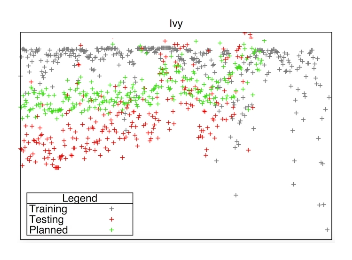
\includegraphics[width=\linewidth]{figs/2d.eps} 
%  % 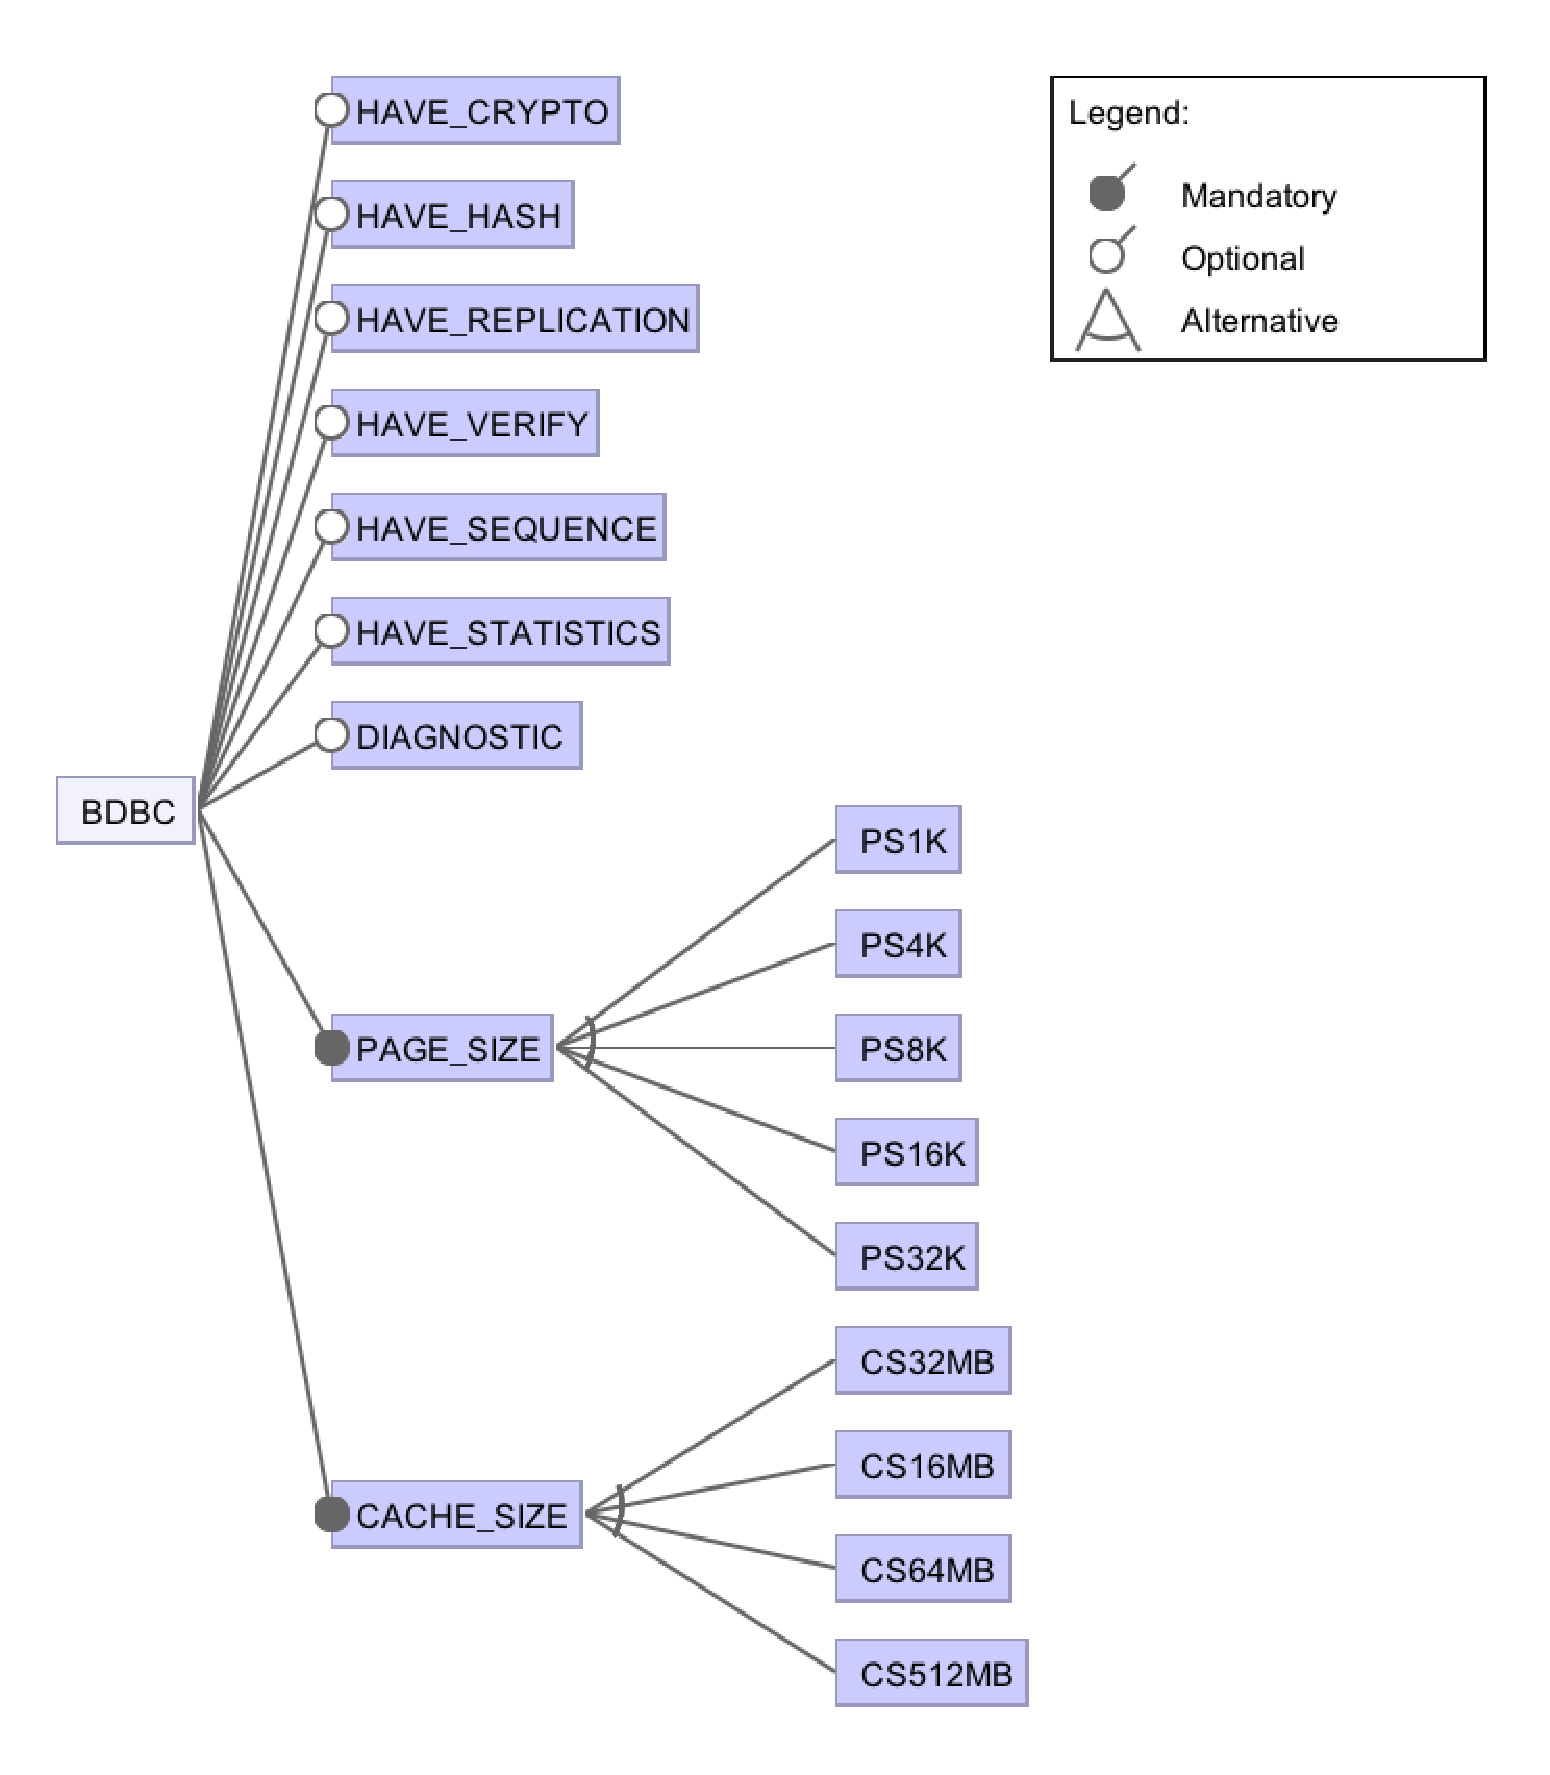
\includegraphics[width=1\linewidth]{figs/BDBC.eps}
% \caption{Gray, red, green show (1) training examples, (2) test examples and 
%   (3) tests that have been altered by planners.
%   This figure uses axes generated from the first two components of a PCA analysis of all points. 
% }\label{fig:howxy}
% \end{figure}
% We should mistrust the predictions made by a  model   if it is being applied to examples  that are
% too far away from the
% training cloud.
% To test for ``too far'', we can run a data mining experiment that tests how well
% a model learned from the training data applies to the test data. Such experiments return some performance value.

% Note that predictions  about changes that  fall within the space of the training+test data, will be at least
% as accurate as the predictions of the original test data. With this, we assert that the predictions for changes that move examples towards/away from the training data can be trusted more/less (respectively).

% Accordingly, we need {\em trust-increasing} planners to generate new examples {\em closer} to the
% training examples.  To see how this works, 
%  \fig{howxy} is from the {\em ivy} data
% set (one of the Jureczko data sets used in this paper). It shows: (1)~the training examples in gray, (2)~the test examples in red, and (3)~the
% changed  examples displaced after applying a plan (in green).
%  Note that the  the   changed examples
% cases  (shown in green)  fall closer to the training cases (shown in gray) than
% the test cases (shown in red). 

% In that green region of changed examples, our belief in the value of predictions
% will be just as much as, if not more than, our belief in the value of the predictions in the red region (that
% contains the original test data).
% This pattern of \fig{howxy} (where the new examples are found closer to  the training cases than the test cases) has been observed in all the other data sets studied in this
% paper. Hence,  we can assert that
% predictors learned from these training examples have some authority in the regions
% containing the changes examples.


% That said, the above comes with some important caveats:
% \bi
% \item 
% The quality of the prediction depends on the nature of the training data. Thus, we strongly recommend that both the data set and the predictor be assessed prior to planning. This ensures that the predictor's performance is adequate for a data set. We tackle this issue in detail in \tion{tesd}.
% \item
% Planners should be designed to be {\em trust increasing}. We list four such planning methods in \tion{planners}.
% \item
% Where possible, planners should be assessed via some external
% oracle that can accurately assess new examples. For an example of that kind of analysis,
% see  \tion{coc}.
% \ei

\subsection{ Learner Bias}
For building the defect predictors in this study, we elected
to use  Random Forests. We chose this approach,  based on its reputation for having the better  performance of 21 other learners for defect prediction~\cite{lessmann}. Data mining is a large and active field and any single study can only use a small subset of the known classification algorithms.  

That said, we have taken care to document in this paper the decisions made by engineering
judgement that could effect our conclusions. The above code used a set of variables which future
work should vary in order to test the internal validity of our conclusions:

\bi
\item The clustering scheme, WHERE, divides data into groups of size $\alpha=\sqrt{N}$;
\item XTREE considered a sibling useful if it's score was less than $\gamma=0.5$ times the mean score of the current leaf.
 \ei

\subsection{  Sampling bias} 
Sampling bias threatens any data mining experiment; i.e., what matters
there may not be true here. For example, the data sets used here comes from two sources
(Seigmund et al. and Jureczko et al.) and any biases in their selection procedures
threaten the validity of these results. 
That said,
the best we can do is define our methods and publicize our data and code so that other researchers can
try to repeat our results and, perhaps, point out a previously unknown bias
in our analysis. Hopefully, other researchers will emulate our methods in
order to repeat, refute, or improve our results. 



\subsection{  Evaluation Bias}\label{sect:coc}
Another threat to validity of this work is our use
of predictors learned on the training data to assess the impact of our planners.
This issue was discussed in detail in \tion{trust}. 

To those notes, we add a few more details. If possible, planners should be assessed via some external oracle that can accurately assess new examples. For example, in search-based software engineering,
examples can be assigned objective scores via  some model. In this approach, a changed example can be assessed by
generating actual objective scores from the model. 

\begin{figure}[!t]
%\noindent\begin{minipage}{0.5\textwidth} 
{\small 
\begin{tabular}{llrrc}
\arrayrulecolor{lightgray}
\rowcolor{lightgray}\textbf{Rank} & \textbf{Treatment} & \textbf{Median} & \textbf{IQR} & \\\hline
  1 &        XTREE &   59   &  9 & \quart{75}{4}{78}{99} \\
2 &      CD &    -9  &  77 & \quart{21}{41}{42}{99} \\
\hline \end{tabular}}
\caption{Planners applied to some ground-truth data (in this case, the POM3 model).
Values collected from  40 repeated runs of each method with different random seeds.
Results show the efficacy of XTREE in reducing the total overall cost in the original test data, when CD fail to do so.}
\label{fig:coc}
\end{figure}

The POM3 model~\cite{boehm2003using},~\cite{port2008} is a tool for exploring management challenges. POM3 implements the Boehm and Turner model of agile programming~\cite{boehm2003balancing} where teams select tasks as they appear in the scrum backlog.  POM3 can study the implications of different ways to adjust task lists in the face of shifting priorities. The model outputs estimated task completion rates; programmer idle rates; and total overall cost. POM3 models requirements as a dependency tree. A single requirement in the tree of a prioritization value has a cost, along with a list of child-requirements and dependencies. Before any requirement can be satisfied, its children and dependencies must first be satisfied. POM3 simulates changing priorities by making teams aware of random items in the requirements tree at random intervals, thus forcing teams to constantly readjust their "to do" lists. For further details on this model see~\cite{boehm2003using},~\cite{port2008}, and~\cite{boehm2003balancing}. 

\fig{coc} shows results from using POM3 as an oracle to assess our planning methods and their ability to reduce the project cost. In this experiment, we generated a training and testing set with 1000 randomly generated instances, which we passed to our four methods.
40 times, we let those methods propose changes to those projects. 
For assessment purposes, the changed projects were then fed back to the POM3
oracle. 

Using this approach, it is possible to assess the value of a plan by measuring its
effectiveness with respect to some ground truth (in this case, the POM3 model).
As shown in \fig{coc}, XTREE reduces the cost by 59\% thereby passing this assessment. These results from the POM3 model further endorse our previous conclusions; i.e. compared to three other methods,  XTREE's supervised methods are best for generating plans on how to change example projects.
 
 
\section{Related work}

\subsection{Planning in AI}

The XTREE planner is somewhat different to the logic-based planners explored by 
classical AI. 
Those kinds of planners employ a logical procedure~\cite{Fikes1971}
that seeks an ordering on {\em operators} to take some domain
{\em state} from a {\em start} state to a {\em  goal} state.
This classical logical approach is known to suffer from
computational bottlenecks~\cite{Bylander1994}. On the other hand, tools like XTREE will scale to any domain
that can generate decision trees.
  
\subsection{Evaluating Changes}

Some organizations have the resources to 
run repeated trials to assess  project changes.
For example, in one   study, Bente et al. reported results
where the same  specification was developed by four different organizations~\cite{Anda2009}. Given those kind of resources, it would be possible
to (say) take a code base, assign it to different teams, make these teams  adopt different polices,
then check in 12 months time
 which teams have fewer defects than the others.  
 

Seldom do industrial or research groups have access
to the kinds of resources needed for this kind study  (evidence: in the six years since the
publication of that work, we know of only one   similar study to Bente et al.). Also, given the
diversity of modern software projects, it might be unreasonable to demand that all
proposed changes for all projects are always evaluated by something like the Bente et al. study.
Hence, this paper has used data miners to build an oracle that can assess changed examples. The advantage
of our approach is that it required far less resources to assess the effectiveness of proposed
changes to a project.  

\subsection{Search-based SE}

Another way way to propose changes to software artifacts
is   via some search-based method~\cite{Harman2009,Harman2011}. Such SBSE methods are   evolutionary programs that 
make
 extensive changes to  some initial sample of project data
 (perhaps 
100s to 100,000s of mutations). Each of these mutations
is reassessed using some domain model.
Examples of these algorithms include GALE, NSGA-II, NSGA-III, SPEA2, IBEA, particle swarm optimization, MOEA/D, etc.~\cite{krall14,deb00a,zit02,zit04,%
deb14,Cui2005a,zhang07:TEC}.

One problem with these   SBSE methods is that they can  make extensive mutations to the data they are exploring. In the language
of \tion{trust}, these methods may not be {\em trust-increasing} since those algorithms make no attempt
to prevent new examples from mutating away from the kinds of data used to commission the model (in which case, we would
start doubting the model's output).

Another issue with standard search-based SE methods is that they require ready access to 
trustworthy domain model that can offer an assessment
of newly generated examples. While some domains have such models (e.g. see the COCOMO effort estimation model
used in the last section), our experience is that many others do not.  For example, 
consider software defect prediction and all the intricate issues that may lead to defects in a product. A model that includes {\em all} those
potential issues would be very large and complex. Further,
the empirical data required to validate any/all parts
of that model can be hard to find.

What we would recommend is a two-pronged policy.
In domains with ready access to trusted models, we recommend
the kinds of tools that are widely used in the search-based
software engineering community such as GALE, NSGA-II, NSGA-III, SPEA2, IBEA, particle swarm optimization, MOEA/D, etc.~\cite{krall14,deb00a,zit02,zit04,%
deb14,Cui2005a,zhang07:TEC}. Otherwise, we recommend tools like XTREE.

\section{Conclusions}

The planner proposed in this paper proposes changes to software project details in order to improve the expected
value of the performance scores of that part of the project.
To evaluate these planners,
data miners can be used to build oracles to assess planners.
Such planners should be {\em trust-increasing}; i.e. they should propose changes that generate
changed examples that are closer to the training data of the data miner.
One caveat here is that the evaluations we can make on the planner are only as good as the predictive
performance of the data miner. Hence, if domain data does not support satisfactory predictors, then
planning in that domain cannot be evaluated.

Four planners were assessed here for the tasks of reducing defects and runtimes. 
Three of the methods come from our prior publications~\cite{me12c,krishna15}, and the conclusion of this
paper is that a novel fourth method clearly out-performs the other three
(measured in terms of {\em effectiveness, succinctness, and surprise}).
We conjecture that XTREE worked better than the rest since:
\bi
\item
It uses a supervised method to divide the data and;
\item
When planning how to move examples to better classes, it is best to reflect over 
differences between those classes.
\ei
\section{Future Work}
Future work in this area could explore numerous questions. For example, 
XTREE, as used here, sought improvements in a one goal (the class variable). Does XTREE work for multi-goal reasoning?

Also, the XTREE algorithm seems quite general to any data of table with rows containing
weighted classes (so we can distinguish ``bad'' rows from ``better'' ones). 
Does   XTREE works  on   domains (other than the defect/runtime data explored here)?

As an example of a domain that might benefit from XTREE, recent results raise doubts about
the value of changing code to remove ``bad smells''~\cite{Sjoberg13}. Can XTREE be used as a ``bad smell'' detector to select the subset of possible refactorings that have the most potential benefit?

As to scalability, XTREE is a post-processor to a decision tree algorithm. Hence, in theory, XTREE   works on domain where data miners can generate decision trees. Given the current state of the art in Big Data, can XTREE  be applied to  very large data sets?
 
We discussed above in \tion{p2p} the general  conclusions of Passos, J{\o}rgensen  et.al~\cite{passos11,jorgensen09};
i.e. software developers are reluctant to surrender their old biases
in the face of new data. 
Accordingly, it must be asked if  the {\em mental resistance} of developers
will prevent them applying XTREE's automatically generated recommendations of tools?
Note this this issue is not just a concern for XTREE, but also for any 
automatic tool proposing refactorings.

There are many more methods for generating plans and
no   one paper can survey them all. For example, this paper has not explored variations to the $\alpha,\beta$, and $\gamma$
parameters that controlled XTREE. Would we get better results if we varied those parameters?

That said, the goal of this paper was not to claim that (e.g.) XTREE is some absolute optimal algorithm. Rather, it is
was to offer a baseline result (with XTREE) and an  evaluation strategy that  can assess  if alternate methods are better than XTREE.
The authors of this paper would actively support other teams exploring this
method (with or without using our current code base). So our last questions is this:
will other  researchers try to repeat and/or improve
(or even refute) our results?  Perhaps.

\section*{Acknowledgements}
The work has partially funded by NSF  award \#1506586.
\bibliographystyle{plain}


\balance
\bibliography{References}
\end{document}


  
  Next, build one centroid for each cluster (using the median and mode value for continuous
and discrete values, respectively).
After that, write a spreadsheet with one column per centroid;
\bi
\item
Sort the columns such that any current projects client fall into the left-most
columns. That is, make the left-hand-side of the sheet  ``current usual practice''
and the right-hand side  ``alternatives to current usual practice''.
\item
Sort the rows of that spreadsheet such that the rows with
maximum  variability appear at the top 
\ei
Now show the sheet to the business user, encouraging them to make recommendations by
\bi
\item
Comparing the left and right-sided columns;
\item
Using the features mentioned in the top-most rows (where changes selects for the most different centroids).
\ei

		
	
		

In theory, One  advantage of this method is that it focuses the attention of the business users
away from rows that do not select for different centroids and towards differences between
current usual practice and everything else.  
In the summer of 2011 and 2012, one of us (Menzies) spent two months
	working on-site at Microsoft Redmond,
	observing data mining analysts.  In that study, he took special
	note about how Microsoft's data scientists
	discussed the results of their data mining sessions with  business users. 
	
	One surprising observation was how  
	little time was spent by business users 
	inspecting  of the output of standard data miners. Prior to that visit,
	we had the mistaken impression that   decision trees,
	clustering algorithms, etc were useful ``off-the-shelf''; i.e    business
	users would inspect and understand the output of those tools.
	
Standard data mining tools are not necessarily the best tool for supporting that dialogue.
Menzies found that he had to do considerable work pre-processing data mining output
prior to the weekly briefing meetings for the business users. Initially,
that pre-processing was just clustering. This evolved into feature selection and finally
the a case-based reasoning tool called HOW.  


	
	as compared to another process, which we call {\em peeking}.
	In {\em peeking}, analysts and users spend much time
	inspecting and discussing small samples of either raw or exemplary or synthesized project data.  Further, very little of those discussions were  focused on classification
	(the addition of a labels to some unlabelled data). Rather, much time
	was spent in those meetings discussing {\em what to do next}; i.e. trying
	to determine what could be altered to better improve some business outcome.
	
	That   Microsoft  study found two common ``peeking'' methods.
	In {\em data engagement meetings},
	users debated the implications of data
	displayed on a screen. In this way, users
	engaged with the data and with each other by
	monitoring each others' queries and check each others'
	conclusions.
	
	Another data analysis pattern observed
	at Microsoft was  {\em cluster + contrast} in which
	data is  reduced to a few
	clusters. Users are then just shown the delta between those
	clusters. While contrasting, if feature values are
	the same in both clusters, then these were pruned from
	the reports to the user. In this way, very large
	data sets can be shown on one PowerPoint
	slide. Note that {\em cluster+contrast} is a tool that can be usefully employed within
	{\em data engagement meetings}.
	
	
	Cluster+contrast and engagement
	meetings are common practices at Microsoft. Yet  these methods had never been rigorously studied or certified.
	For both those reasons,
	we reflected over those tools to discover and analyze their
	underlying process. The result was HOW~\cite{howase}: a tool
	that combines (a)~feature selection; (b)~centroid generation from   clusters;
	(c)~contrast methods between centroids.
	While method (a) is widely used (e.g.~\cite{Menzies2010}),
	to the best of our knowledge, this combination of (abc) has not been thoroughly explored before.

This paper assesses two methods  for ``peeking'': a model-based method called DTREE and an instance-based method   called HOW. 
DTREE were first developed by Lekkalapudi and Menzies to  explaining results from multi-objective optimizers~\cite{nva14}. This paper is the first
to apply DTREE to defect prediction and contrast set learning. Also, that prior work evaluated
DTREE against multi-objective optimizers and not   instance-based methods.

This paper uses three criteria to assess the value of HOW and DTREE for
learning actionable analytics:
\be
\item
A planning system needs to be {\em effective}; i.e. if its recommendations
are applied then some statistically significant change should be observed.
To predict the number of defects in a data set before and after applying our changes,
we build a    prediction system (built by data mining; specifically: Random Forest). Note that this
predictor was built from some hold-out data (i.e. from  different data than that used
to build the predictor).
\item
Any  conclusion made to a business user must be understandable;
it must generate {\em succinct} changes.  
\item
Recommendations should be {\em stable}; i.e. they shouldn't widely vary due to minor changes in the data. Hence, in our experiments, we will add a little randomness to our analysis then report results across 20 repeated runs. 
\ee
We will find that
 {\em effectiveness} of DTREE and HOW are similar, but   DTREE wins on {\em succinctness} and {\em stability}.

\section{Cluster and Contrast}
\label{clust_contrast}
A recurring data analysis pattern in this paper is $cluster+contrast$. The data is distilled into a few clusters using a clustering scheme. Then lessons are inferred by studying the differences between these clusters. These lessons are used to generate rules that can be applied in any context.

\subsection{Clustering}
There are a wide variety of clustering methods to choose from. A study by Ganesan~\cite{div14} explored different clustering methods for software engineering data using the effort and Jureczko data from the PROMISE repository~\cite{promise}. In that study methods such as WHERE, K-Means, mini-batch-K-Means, DBScan, EM, and Ward were investigated. The results of the study showed that the size and number of clusters is more important that the specifics of the techniques used. 

For this purposes of this work, we have chosen WHERE, a clustering scheme which is capable of generating at least $\sqrt{N}$ clusters given $N$ instances. In addition to this, WHERE has been shown to run fast while ignoring spurious dimensions~\cite{menzies2013}. This is particularly useful, for much of the SE data is noisy, they contain a information not associated with the target variable. 

\subsection{Finding Contrasts}
All the following methods use clustering in the form of WHERE, a top-down clustering method which recursively splits the data in two along a dimension that represents the highest variability. It works as follows:
\bi
\item Find   two   distance samples from the data, say  $X,Y$. This can be done by  picking any case $W$ at random, then setting $X$ to its most distant case, then setting $Y$ to the case most distant from $X$ (this requires only $O(2N)$ comparisons of $N$ cases).
\item Project each case $Z$ onto a {\tt Slope} that  runs between $X,Y$ using the cosine rule. 
\item Split the data at the median $X$ value of all cases and recurse on each half  (stopping when one half has less  than $\sqrt{N}$ of the original population).
\ei		

Clustering is followed by generating \textit{contrast sets}. These contrast sets represent recommendations on what could be altered to better improve an outcome. In this work we have explored several algorithms as possible tools to identify contrast between clusters. These fall into two broad categories:
\begin{enumerate}
\item Case Based Reasoning techniques (Nearest Neighbors and a gradient base planner called HOW)
\item Decision Trees.
\end{enumerate}

These techniques are discussed below. It is worth noting that the following techniques are organized in such a way that each one seeks to address certain shortcomings in the ones that precede it. 

\subsection{Case Based Reasoning}

Case-based reasoning seeks to find solutions to problems by emulating human recollection and adaptation from past experiences. It has found extensive usage in Artificial Intelligence because it offers several advantages. However, one of the most important benefits that CBR has to offer is that it works on a ``case-by-case'' basis. Therefore it's advise is tailored to be specific to the particular case being considered. Several paper in SE have applied this technique, most of all for effort estimation ~\cite{keung2008analogy, 6600685, walkerden1999empirical, shepperd1997estimating, kocaguneli2010use}. 

A classic example of a CBR is K Nearest Neighbor. Our version of nearest neighbor for planning is rather straight forward. It has been developed as a "straw-man"; i.e., a simple baseline tool to act as a benchmark used to evaluate other methods. 


\subsection{HOW}

HOW is very different compared to conventional CBR planners in that it explores the gradient between pairs of nearby clusters instead of studying the clusters themselves. HOW works by clustering the data during training using WHERE and then drawing \texttt{slopes} between the centroids of pairs of nearby clusters. Assuming the cluster pairs are labeled X and Y, with X having slightly better performance score than Y, the \texttt{slope} between X and Y acts as an indicator pointing to a direction in which to displace the data; i.e. away from Y and towards X. 

While testing, HOW finds the nearest slope to every test case. The slope provides the exact magnitude and direction of displacements. Contrast sets are derived from these displacements. HOW offers a distinct advantage over the other CBR planners by limiting the displacements to very small regions (the displacements are never more than the separation between two clusters). 

Although HOW manages to generate plans by localizing displacements to regions small enough to produce a statistically significant improvement, it needs to be noted that it fails to provide succinct summaries. Lack of succinctness makes it difficult draw generalizable conclusions about the test data. This is a trend commonly observed in most CBR systems. They tend to reason directly from a loaded training data instead of first summarizing the data into a model. 

% However, not all domains come with reliable models. For instance, a model that encompasses all the intricate issues that may lead to defects in software would be very large and indeed rather complex. In addition to this, finding empirical data to validate such models can be hard to come by and also time consuming ~\cite{me09i,me09j}. 

\subsection{DECISION TREES}

Trustworthy domain models are a popular alternatives to CBR planners. In our previous work, we have used executing source code as a "model" to check if our mutations to test suites minimize the test suite size while maximizing the number of statements covered~\cite{me09m,andrews07,andrews10}. However, we do not always have access to ready-to-use models. Further, finding empirical data to validate existing models can be hard. 

Taking into account the wealth of data that is available to us, this issue can fortunately be circumvented by constructing a categorical model based on decision trees. Unlike the previous planners which use where, here we construct a decision tree using information gain as a metric to find ideal splits in the data. This allows us to identify the most informative attributes to select. A decision tree (hereafter referred to as DTREE) built in this fashion emulates a model built from the training data. 

Using DTREE, the test cases can be categorized into one of the branches of the tree. Now, to generate the contrast sets, we determine (1) What \textit{current} branch does a test case fall in?; (2) What \textit{desired} branch would the test case have to move to?; (3) What are the deltas between \textit{current} and \textit{desired}? The last question can be answered by finding the deltas in branches of the decision tree that lead to \textit{desired} from \textit{current}. For full algorithmic details, refer to \fig{xtrees_bare}.

A tree structure such as DTREE is characterized by attributes such as size and depth. It is worth noting that these attributes have a profound impact on its performance. Our initial motivation for using DTREE was that they could serve as a medium for experts to reason about a data. The size of the tree, if too large, jeopardizes the readability of the solutions by increasing the complexity. We have, therefore, endeavored to reduce the size of the tree by pruning away irrelevant solutions that do not contribute to better solutions (refer to step-2 of \fig{xtrees_bare}). 

DTREE offers a great number of benefits compared to the other methods that were discussed above. Firstly, it offers a visual medium for experts to identify and explore solutions spaces that are local to the problem. Secondly, its solutions are much more stable than other cluster specific and instance specific learners. This stability can be attributed to the consistency and general reproducibility of the tree structure. Thirdly, and perhaps most importantly, the tree summarizes the training data succinctly, making it easier for a business user to examine the solution sets.

\lstnewenvironment{code}[1]{
\lstset{
mathescape,
numbers=left,
numberstyle=\scriptsize,
stepnumber=1,
numbersep=0.5em,
xleftmargin=1em,
framextopmargin=2em,
framexbottommargin=2em,
showspaces=false,
showtabs=false,
showstringspaces=false,
tabsize=2,
% Basic
basicstyle=\ttfamily\scriptsize,
backgroundcolor=\color{Background},
language=Python,
% Comments
commentstyle=\color{Comments}\slshape,
% Strings
stringstyle=\color{Strings},
morecomment=[s][\color{Strings}]{"""}{"""},
morecomment=[s][\color{Strings}]{'''}{'''},
% keywords
morekeywords={[1]import,from,class,def,for,while,if,is,in,elif,else,not,and,or,print,break,continue,return,True,False,None,access,as,,del,except,exec,finally,global,import,lambda,pass,print,raise,try,assert, dot, norm, zip, sorted},
keywordstyle={[1]\color{Code}\bfseries},
% additional keywords
morekeywords={[3]fastmap,Slope,bPruning,clister,train,leafs,weightedFeatures,HOW,envy, score,kNN,contrastSet,exemplar,Prune, FSel, exemplar,nearestSlope,dist,displace,geometry,splitAcross2Points,leaves,How,nearest,bPruning,Stats,divide,recurse,weight1,project, furthest, split,WHERE,clusterer, getContours,envied, fWeight, nearestContour, projection, mutate, HERE, knn},
keywordstyle={[3]\color{Keywords}\bfseries},
morekeywords={[2]@invari},
keywordstyle={[2]\color{Decorators}\slshape},
emph={self},
emphstyle={\color{self}\slshape},
firstnumber=last
%
}}{}




It turns out that ranking codiiiiie smells, and ignoring the low priority
ones, is a pressing problem. As shown in our {\em Related Work} section,
different developers and  books and tools stress the importance of different code smells. How to assess these different claims? How to avoid
needless refactoring? How to check if a code smell found at another site
is relevant to this site?

To answer all these questions, we propose NOSE, a tool that checks
if cpde smells really smell 
generates candidate refactorings to reduce the chances of software
defects. XTREE is a back-end to a decision tree learner that
reflects on how different branches in that tree predict for
defective or non-defective code modules. Since this tree
is built from static code attributes, the differences between
those brnachesy reflecting on the
{\em delta} between those branches, it is 







When modern software systems are developed, their design 
changes continuously. Due to market constraints, the developers tend to ignore the quality of source code, thereby introducing \textit{code smells} (or \textit{anti-pattern}). These anti-patterns are generally viewed as poor solutions to recurring design problems, possibly deterring the maintainability of the system. In the past decade there has been growing evidence of the impact of anti-patterns, there now is also some empirical evidence to suggest that code containing anti-patterns are more fault prone than the rest of the code~\cite{khomh12}\cite{li07}\cite{fab15_1}. Studies show that the number of code smells increase over time and in only a very few cases are these smells addressed by refactoring \cite{fab15_1}\cite{chatzigeorgiou10}\cite{arcoverde11}. This makes early detection of these code smells a necessity to maintain sufficient quality in software systems. This being said, detection only addresses a part of the problem, what we need are recommendation systems that can assist a software developed not only by identifying potential anti-patterns, but also by (i) generating reliable refactoring options, and (ii) critiquing bad refactoring options. 

Tools for detecting code smells have been the focus of several researchers lately, \cite{Tufano2015}\cite{boussaa13}. There are two  popular techniques for detecting smells: (1) by the making use of static code analysis and code quality metrics\cite{tsantalis09}; (2) Analysing software change history\cite{moha2010}. While these tools are capable of detecting these smells with a reasonable accuracy, they fail to provide developers with planning actions to improve the quality of source code.  Similar concerns were voiced by several business users, who are demanding tools that support business-level interpretations of their data. 

At a panel on software analytics at ICSE`12, industrial practitioners lamented the state of the art in software analytics~\cite{menzies12a}. Panelists commented  ``prediction is all well and good, but what about decision making?''. The panelists were more interested in the interpretations and follow-up that occurs after the mining, rather than just the mining itself. We call such tools \textit{planners}. In the context of detecting code smells, the planners are required to address the following issues.

\bi
\item
Instead of just \textit{detecting} anti-patterns and code smells, it may be beneficial to develop tools that can be used to reason about the code smells. 
\item
In addition to detecting anti-patterns and code smells, tools must be capable of having a contextual understanding of the data to trigger only the most useful refactoring options.
\item Tools must provide a visual medium for developer to gauge the nature of refactoring options, thereby discarding bad solutions.
\ei

In response to this, we propose a novel {\em planning} method called XTREE which reflects on static code quality metrics to learn refactoring options to a software system such that its performance ``improves'' quantitatively. As a measure of source code quality we take into account the number of classes with defects in them. To this end, we use defect count data set by Jureczko et al. for JAVA systems~\cite{jureczko10}. In addition to defects, the aforementioned data set measures a list of static code attributes associated with each class. These code attributes allow us to reason about the measurable properties of anti-patterns. 

The contributions of this paper are (1) the new XTREE planning algorithm and (2) an evaluation strategy that shows the tool performing significantly ``better'' than  the  planner  proposed in our prior work~\cite{me12c}. 

The work on XTREE is motivated by the following three research questions:

\bi
\item \textbf{RQ1:} \textit{Can a planner suggest plans to improve the quality of a defective class?} This research question investigates the effectiveness of a planner in suggesting useful refactoring options to improve the quality of class by reducing the number of defects. Specifically, we use XTREE to suggest a number of valid changes to source code and we use an oracle to measure the effectiveness of the changes, see \tion{eval}. In order to ensure the changes are feasible, XTREE generate succinct plans.

\item \textbf{RQ2:} \textit{Can a planner be used to critique bad refactoring options?} In addition to being able to suggesting changes, it's beneficial for planners to be able to quantitatively comment on the quality of certain refactoring options, thereby preventing unnecessary refactoring.

\ei

The rest of this paper  describes our data, our planners, and the experiment that ranks XTREE against alternate approaches.  This is followed by notes on related work and validity. To enable reproducibility, all scripts and data used in this study are available online at \url{http://git.io/vG3DG}.

Fowler claims   removing   code smells   by
\begin{quote}
...applying a series of small behavior-preserving transformations, each 
of which seem ``too small to be worth doing''. 
The  effect of   these transformations is quite significant. By doing them in small steps you {\em reduce the risk of introducing errors}'' (our italics).
\end{quote}
The italics in the last paragraph offer one method for indicating if bad smell-based
refactoring was successful. There are many automatic
methods for learning   defect predictors from static
code features~\cite{peters15,he13}.  We can use those
predictors to rank $N$ proposed refactorings $R_1,R_2,...R_i$
refactorings. Specifically, we  say that refactoring $i$ is preferred to $j$
(denoted $R_i \succ R_j$) if the defect predictors predict fewer errors
after applying $R_i$ than $R_j$.


The ability to rank, and perhaps   reject, a proposed refactoring is
an important contribution, given the current level of interest
in bad smell-based refactoring.


Nevertheless,
certain results raise doubts about the value of   code smells for reducing the risk of defects in software.
